% Options for packages loaded elsewhere
\PassOptionsToPackage{unicode}{hyperref}
\PassOptionsToPackage{hyphens}{url}
\PassOptionsToPackage{dvipsnames,svgnames,x11names}{xcolor}
%
\documentclass[
]{agujournal2019}

\usepackage{amsmath,amssymb}
\usepackage{iftex}
\ifPDFTeX
  \usepackage[T1]{fontenc}
  \usepackage[utf8]{inputenc}
  \usepackage{textcomp} % provide euro and other symbols
\else % if luatex or xetex
  \usepackage{unicode-math}
  \defaultfontfeatures{Scale=MatchLowercase}
  \defaultfontfeatures[\rmfamily]{Ligatures=TeX,Scale=1}
\fi
\usepackage{lmodern}
\ifPDFTeX\else  
    % xetex/luatex font selection
\fi
% Use upquote if available, for straight quotes in verbatim environments
\IfFileExists{upquote.sty}{\usepackage{upquote}}{}
\IfFileExists{microtype.sty}{% use microtype if available
  \usepackage[]{microtype}
  \UseMicrotypeSet[protrusion]{basicmath} % disable protrusion for tt fonts
}{}
\makeatletter
\@ifundefined{KOMAClassName}{% if non-KOMA class
  \IfFileExists{parskip.sty}{%
    \usepackage{parskip}
  }{% else
    \setlength{\parindent}{0pt}
    \setlength{\parskip}{6pt plus 2pt minus 1pt}}
}{% if KOMA class
  \KOMAoptions{parskip=half}}
\makeatother
\usepackage{xcolor}
\setlength{\emergencystretch}{3em} % prevent overfull lines
\setcounter{secnumdepth}{5}
% Make \paragraph and \subparagraph free-standing
\makeatletter
\ifx\paragraph\undefined\else
  \let\oldparagraph\paragraph
  \renewcommand{\paragraph}{
    \@ifstar
      \xxxParagraphStar
      \xxxParagraphNoStar
  }
  \newcommand{\xxxParagraphStar}[1]{\oldparagraph*{#1}\mbox{}}
  \newcommand{\xxxParagraphNoStar}[1]{\oldparagraph{#1}\mbox{}}
\fi
\ifx\subparagraph\undefined\else
  \let\oldsubparagraph\subparagraph
  \renewcommand{\subparagraph}{
    \@ifstar
      \xxxSubParagraphStar
      \xxxSubParagraphNoStar
  }
  \newcommand{\xxxSubParagraphStar}[1]{\oldsubparagraph*{#1}\mbox{}}
  \newcommand{\xxxSubParagraphNoStar}[1]{\oldsubparagraph{#1}\mbox{}}
\fi
\makeatother


\providecommand{\tightlist}{%
  \setlength{\itemsep}{0pt}\setlength{\parskip}{0pt}}\usepackage{longtable,booktabs,array}
\usepackage{calc} % for calculating minipage widths
% Correct order of tables after \paragraph or \subparagraph
\usepackage{etoolbox}
\makeatletter
\patchcmd\longtable{\par}{\if@noskipsec\mbox{}\fi\par}{}{}
\makeatother
% Allow footnotes in longtable head/foot
\IfFileExists{footnotehyper.sty}{\usepackage{footnotehyper}}{\usepackage{footnote}}
\makesavenoteenv{longtable}
\usepackage{graphicx}
\makeatletter
\def\maxwidth{\ifdim\Gin@nat@width>\linewidth\linewidth\else\Gin@nat@width\fi}
\def\maxheight{\ifdim\Gin@nat@height>\textheight\textheight\else\Gin@nat@height\fi}
\makeatother
% Scale images if necessary, so that they will not overflow the page
% margins by default, and it is still possible to overwrite the defaults
% using explicit options in \includegraphics[width, height, ...]{}
\setkeys{Gin}{width=\maxwidth,height=\maxheight,keepaspectratio}
% Set default figure placement to htbp
\makeatletter
\def\fps@figure{htbp}
\makeatother
% definitions for citeproc citations
\NewDocumentCommand\citeproctext{}{}
\NewDocumentCommand\citeproc{mm}{%
  \begingroup\def\citeproctext{#2}\cite{#1}\endgroup}
\makeatletter
 % allow citations to break across lines
 \let\@cite@ofmt\@firstofone
 % avoid brackets around text for \cite:
 \def\@biblabel#1{}
 \def\@cite#1#2{{#1\if@tempswa , #2\fi}}
\makeatother
\newlength{\cslhangindent}
\setlength{\cslhangindent}{1.5em}
\newlength{\csllabelwidth}
\setlength{\csllabelwidth}{3em}
\newenvironment{CSLReferences}[2] % #1 hanging-indent, #2 entry-spacing
 {\begin{list}{}{%
  \setlength{\itemindent}{0pt}
  \setlength{\leftmargin}{0pt}
  \setlength{\parsep}{0pt}
  % turn on hanging indent if param 1 is 1
  \ifodd #1
   \setlength{\leftmargin}{\cslhangindent}
   \setlength{\itemindent}{-1\cslhangindent}
  \fi
  % set entry spacing
  \setlength{\itemsep}{#2\baselineskip}}}
 {\end{list}}
\usepackage{calc}
\newcommand{\CSLBlock}[1]{\hfill\break\parbox[t]{\linewidth}{\strut\ignorespaces#1\strut}}
\newcommand{\CSLLeftMargin}[1]{\parbox[t]{\csllabelwidth}{\strut#1\strut}}
\newcommand{\CSLRightInline}[1]{\parbox[t]{\linewidth - \csllabelwidth}{\strut#1\strut}}
\newcommand{\CSLIndent}[1]{\hspace{\cslhangindent}#1}

\usepackage{url} %this package should fix any errors with URLs in refs.
\usepackage{lineno}
\usepackage[inline]{trackchanges} %for better track changes. finalnew option will compile document with changes incorporated.
\usepackage{soul}
\linenumbers
\makeatletter
\@ifpackageloaded{float}{}{\usepackage{float}}
\floatstyle{plain}
\@ifundefined{c@chapter}{\newfloat{suppfig}{h}{losuppfig}}{\newfloat{suppfig}{h}{losuppfig}[chapter]}
\floatname{suppfig}{Figure S}
\newcommand*\quartosuppfigref[1]{Figure \hyperref[#1]{S\ref{#1}}}
\@ifpackageloaded{caption}{}{\usepackage{caption}}
\DeclareCaptionLabelFormat{quartosuppfigreflabelformat}{#1#2}
\captionsetup[suppfig]{labelformat=quartosuppfigreflabelformat}
\newcommand*\listofsuppfigs{\listof{suppfig}{List of Supplementary Figures}}
\makeatother
\makeatletter
\@ifpackageloaded{caption}{}{\usepackage{caption}}
\AtBeginDocument{%
\ifdefined\contentsname
  \renewcommand*\contentsname{Table of contents}
\else
  \newcommand\contentsname{Table of contents}
\fi
\ifdefined\listfigurename
  \renewcommand*\listfigurename{List of Figures}
\else
  \newcommand\listfigurename{List of Figures}
\fi
\ifdefined\listtablename
  \renewcommand*\listtablename{List of Tables}
\else
  \newcommand\listtablename{List of Tables}
\fi
\ifdefined\figurename
  \renewcommand*\figurename{Figure}
\else
  \newcommand\figurename{Figure}
\fi
\ifdefined\tablename
  \renewcommand*\tablename{Table}
\else
  \newcommand\tablename{Table}
\fi
}
\@ifpackageloaded{float}{}{\usepackage{float}}
\floatstyle{ruled}
\@ifundefined{c@chapter}{\newfloat{codelisting}{h}{lop}}{\newfloat{codelisting}{h}{lop}[chapter]}
\floatname{codelisting}{Listing}
\newcommand*\listoflistings{\listof{codelisting}{List of Listings}}
\makeatother
\makeatletter
\makeatother
\makeatletter
\@ifpackageloaded{caption}{}{\usepackage{caption}}
\@ifpackageloaded{subcaption}{}{\usepackage{subcaption}}
\makeatother

\ifLuaTeX
  \usepackage{selnolig}  % disable illegal ligatures
\fi
\usepackage{bookmark}

\IfFileExists{xurl.sty}{\usepackage{xurl}}{} % add URL line breaks if available
\urlstyle{same} % disable monospaced font for URLs
\hypersetup{
  pdftitle={Regional Base-Flow Index in Arid Landscapes Using Machine Learning and Instrumented Records},
  pdfauthor={Caelum Mroczek; Abraham Springer; Neha Gupta; Benjamin Lucas},
  pdfkeywords={Base Flow, Base-flow Index, Regionalization, Machine
Learning},
  colorlinks=true,
  linkcolor={blue},
  filecolor={Maroon},
  citecolor={Blue},
  urlcolor={Blue},
  pdfcreator={LaTeX via pandoc}}


\journalname{Water Resources Research}

\draftfalse

\begin{document}
\title{Regional Base-Flow Index in Arid Landscapes Using Machine
Learning and Instrumented Records}

\authors{Caelum Mroczek\affil{1}, Abraham Springer\affil{1}, Neha
Gupta\affil{2}, Benjamin Lucas\affil{3}}
\affiliation{1}{School of Earth and Sustainability, Northern Arizona
University, Flagstaff, AZ, USA, }\affiliation{2}{Department of Hydrology
and Atmospheric Sciences, University of Arizona, Tucson, AZ,
USA, }\affiliation{3}{Department of Mathematics and Statistics, Northern
Arizona University, Flagstaff, AZ, USA, }
\correspondingauthor{Caelum Mroczek}{csm428@nau.edu}


\begin{abstract}
Base flow, sustained by groundwater discharge, is a vital component of
river ecosystems, particularly in drylands, where water resources are
limited. This study analyzes the instrumented streamflow record in
Arizona to assess long-term base-flow index (BFI) trends across gauged
catchments. Results indicate that approximately 32\% of Arizona's
streamflow originates from groundwater discharge, with significant
spatial variability driven by landscape and climatic factors. Base flow
relationships are analyzed with coincident trends in climate variables
such as precipitation, evapotranspiration, and temperature. Spatial and
climatic trends reveal variability in base-flow contributions, providing
insight into groundwater-surface water interactions in arid and
semi-arid landscapes. Building on this analysis, we applied machine
learning methods to predict BFI in ungauged basins, addressing the
challenges of Arizona's sparse streamgage network. Using the eXtreme
Gradient Boosting (XGBoost) algorithm trained on hydroclimate and
physiographic predictors, we estimated long-term BFI from 1991 to 2020.
This combined approach integrates observational data with predictive
modeling to enhance our understanding of base-flow processes and provide
a framework for water resource management in data-limited regions.
\end{abstract}

\section*{Plain Language Summary}
Rivers in drylands, such as Arizona, depend on groundwater contributions
to maintain flow during dry periods. This portion of streamflow, called
base flow, plays a critical role in supporting ecosystems and water
availability in these regions. This study examines long-term patterns of
base flow in Arizona using data from streamflow monitoring stations. We
found that about 32\% of Arizona's river flow comes from groundwater,
though this varies significantly across the state depending on local
climate and landscape features. We also analyzed how base flow is
influenced by changes in precipitation, evapotranspiration, and
temperature, providing insights into how groundwater and surface water
interact in these complex environments. To estimate base flow in basins
without monitoring stations, we used machine learning techniques. By
training a model on data from monitored sites and corresponding
hydroclimate data, we predicted long-term base flow for ungauged areas
across Arizona. This innovative approach addresses the challenge of
Arizona's sparse monitoring network and provides a valuable tool for
understanding and managing water resources in regions with limited data.




\section{Introduction}\label{sec-intro}

Dryland regions, encompassing arid, semi-arid, hyper-arid, and dry
sub-humid systems, account for 40\% of the Earth's land surface. These
regions are home to approximately 2 billion people globally and
constitute the largest terrestrial biome (IUCN, 2019). Despite
supporting diverse ecosystems and human populations, dryland regions
face mounting hydrologic challenges exacerbated by increasing
urbanization, expanding agricultural activities, and climate-induced
amplification of precipitation patterns (Taylor et al., 2013). This
water scarcity is intensifying due to the compounding effects of climate
variability and increased groundwater extraction (Taylor et al., 2013).
In drylands, groundwater serves as a vital resource for sustaining
ecosystems and meeting human needs (Scanlon et al., 2006; Yao et al.,
2018).

Base flow is the sustained portion of streamflow in the absence of
runoff that is derived from groundwater discharge (USGS, 2018). Base
flow is critical to maintaining seasonal low-flow regimes, supporting
aquatic ecosystems, and facilitating the transport of nutrients and
chemicals. Base-flow contribution to streamflow can be highly variable
spatially (Beck et al., 2013; Bosch et al., 2017; Singh et al., 2018),
and temporally (Ficklin et al., 2016; Tan et al., 2020). Increasing
groundwater extraction, changes in land cover/land use, and changes in
precipitation patterns due to climate change affect the timing and
volumes of base flow (Tan et al., 2020; Taylor et al., 2013). Effective
management of water quantity and quality depends on understanding
seasonal and interannual base-flow patterns and long-term changes in
base-flow behavior.

The Base-Flow Index (BFI) is the ratio of the long-term mean base-flow
volume to the long-term total streamflow volume expressed as a
percentage. BFI serves as a normalized measure of groundwater
contribution interannually or between basins. BFI is determined by
hydrograph separation and is influenced by the climate and physiographic
characteristics of a catchment (Beck et al., 2013; Neff et al., 2005;
Singh et al., 2018). Between catchments, base flow fluctuates according
to changes in the moisture content of the vadose zone, influenced by
varying levels of evapotranspiration and aquifer storage dynamics (Bosch
et al., 2017). Since BFI calculations rely on instrumented stream
records, it remains unknown for ungauged catchments, which encompass
most of the earth's land surface (Fekete et al., 2007). Addressing this
information gap is integral to approaching a comprehensive understanding
of groundwater dynamics globally.

Advancements in machine learning provide tools to predict hydrologic
indices in ungauged basins, addressing the limitations of sparse
streamgage networks. To tackle the challenge of quantifying base flow in
ungauged catchments, numerous studies have applied both regression and
machine learning methods. Ahiablame et al. (2013) found that using a
regression model to estimate annual base flow of ungauged catchments was
reasonably easy and accurate. Beck et al. (2013) overcame the
nonlinearity of basin characteristics and improved results of
multivariate analyses by using artificial neural networks to estimate
BFI globally. Singh et al. (2018) implemented a random forest algorithm
to predict long-term BFI for ungauged catchments across New Zealand.
These applications demonstrate the versatility and effectiveness of
machine learning in capturing complex ecohydrologic dynamics and
improving our understanding of groundwater contributions to streamflow.

This study develops a technique for estimating BFI in ungauged basins
across Arizona and evaluates the state's long-term BFI. Regional trends
in base flow and BFI at instrumented sites are also analyzed, with these
trends being linked to coincident trends in precipitation,
evapotranspiration (ET\textsubscript{O}), and temperature over the same
periods. Using a machine learning model trained on the hydrogeologic
characteristics of surface water basins, we estimate the mean BFI for
ungauged basins from 1991 to 2020. This approach helps address the
spatial gaps in the streamgage network, which is relatively sparse
across the state. The results offer novel insights into low-flow
processes in both gauged and ungauged basins, enhancing our
understanding of climate controls on consistent flows in Arizona. This
study contributes to a more comprehensive view of hydrological dynamics
in the context of arid and semi-arid landscapes.

\section{Data \& Methods}\label{sec-data-methods}

\subsection{Study Area}\label{sec-study-area}

The state of Arizona, located in the southwest United States, covers a
total area of 295,253 km\(^2\). Arizona is divided into two primary
physiographic provinces: the Colorado Plateau in the northeast, and the
Basin-and-Range region in the west and south. The Central Highlands is a
transition zone consisting of scattered basins separated by the
mountainous foothills of the Mogollon Rim. The Colorado Plateau is
dominated by high-elevation desert with an average elevation of 1,936
masl (6,352 ft). Mean temperatures range from -6\(^\circ\)C
(20\(^\circ\)F) to 26\(^\circ\)C (80\(^\circ\)F) and it averages 580 mm
(23 in) of precipitation. The Basin-and-Range region has a semi-arid to
arid climate with an average elevation of 490 masl (1600 ft). Average
temperature ranges from 15\(^\circ\)C (60\(^\circ\)F) to 43\(^\circ\)C
(110\(^\circ\)F) and the region averages 200 mm (8 in) of precipitation
annually (Arizona State Climate Office, 2024).

\begin{figure}

\centering{

\includegraphics{images/StudyArea_20241203.png}

}

\caption{\label{fig-study-area}Map of Arizona indicating US Geological
Survey (USGS) streamgages used in this study. 8-digit HUC subbasin
boundaries and physiographic regions shown.}

\end{figure}%

Arizona's hydrology varies seasonally and spatially between its
physiographic regions. In the summer, localized and intense convective
precipitation events are driven by the North American Monsoon, while in
the winter, orographic precipitation comes from Pacific frontal systems
(Eastoe et al., 2019). While monsoonal precipitation can account for up
to 50\% of annual precipitation, evaporation and dry preceding soil
properties leads to most precipitation becoming runoff (Sheppard et al.,
2002). As such, 94\% of streams in Arizona are ephemeral or intermittent
(Levick et al., 2008). Much of the hydrology of Arizona is snow-melt
derived, driven by spring melt from the high-elevation Colorado Plateau
winter snowpack. While winter precipitation provides only 30\% of annual
averages, it provides the majority of water for natural reservoirs
(Sheppard et al., 2002).

\subsection{Data}\label{sec-data}

Daily observed streamflow data obtained from the United States
Geological Survey (USGS) National Water Information System (NWIS) were
used in this study. Streamgages were selected depending on criteria to
ensure the applicability of each site. Following the findings of
O'Donnell et al. (2016), which determined that 8--10 years of
calibration data are necessary to account for climate variability in
paired watershed studies in the region, a minimum record length of 10
years was required. Additionally, years with more than 30 missing days
of streamflow data were excluded from the analysis. This study focuses
on natural, streamflow-influencing dynamics, so streamgages affected by
regulation or diversions were excluded. The regulated river streamgages
were identified through annual reports on water data published by the
USGS (USGS, 2010). Furthermore, streamgages along the Colorado River
were omitted because they represent managed flows governed by the
Colorado River Compact. After applying these selection criteria, 205
USGS streamgages with acceptable periods of record were included in the
study (Figure~\ref{fig-study-area}). Periods of record ranged from 10 to
112 years, with a median of 28 years.

While our data selection ensures a robust record for this analysis, it
also highlights gaps in spatial coverage that the machine learning model
can address. Arizona has 184 active USGS streamflow stations (as of
2024) across an area of 295,253 km², whereas Indiana (a humid state in
the U.S.) has 189 active stations within an area of 94,326 km². This
translates to a streamgage density of approximately 2.004 gages per
1,000 km² in Indiana, over three times higher than Arizona's density of
0.623 gages per 1,000 km². This stark difference underscores the
relative sparsity of Arizona's streamgage network, particularly in the
context of its larger geographic area and the unique hydrological
challenges posed by its arid and semi-arid landscapes.

Watersheds across the United States are delineated by the USGS using a
hydrologically-defined network. This system delineates the country using
hierarchical hydrologic unit codes (HUCs), where each subsequent basin
includes the digits of the enclosing basin. Here, 8-digit HUCs (HUC 8s)
are used to divide Arizona into 84 sub-basins that are fully or
partially in the state (Figure~\ref{fig-study-area}). These HUC 8
sub-basins are analogous to medium-sized river basins and are defined by
surface water characteristics.

Annual precipitation and temperature data came from the PRISM climate
group at Oregon State University at a resolution of 4 km
(\url{https://prism.oregonstate.edu;} (Daly et al., 2008)). The PRISM
dataset provides valuable insights into regional climate in ungauged
regions and has been shown to perform well across the southwestern US
(Buban et al., 2020). Instead of the water year, PRISM data uses a
calendar-year format, which was adopted for consistency in the water
balance. Although this may introduce challenges in the annual estimates
due to inter-annual snow storage, the use of long-term annual averages
is likely to reduce any potential errors (Reitz et al., 2017).

Annual reference evapotranspiration (ET\textsubscript{O}) data came from
TerraClimate, a 4-km grid climatalogical data set (Abatzoglou et al.,
2018). TerraClimate uses a Penman-Monteith approach to generate a
reference evapotranspiration. The ET\textsubscript{O} values were
calculated assuming a reference grass surface across the landscape with
unlimited water. In the drylands of the southwestern US,
ET\textsubscript{O} typically exceeds precipitation annually (Zomer et
al., 2022).

A 30-meter resolution Digital Elevation Model (DEM) of Arizona was used
to derive key basin characteristics: basin area, average slope, and the
proportion of each basin oriented toward north or south aspects. Various
geospatial variables, such as aspect, were disaggregated then averaged
to assess the areal percentage of each sub-variable within individual
HUC 8 basins. By calculating these percentages, we aimed to get a more
comprehensive understanding of landscape composition across space. Land
cover was acquired from USGS-NLCD (National Land Cover Database),
hydrologic soil group from SSURGO (Soil Survey Geographic Database), and
underlying geology and karst from USGS were all similarly averaged
across the basins. Aggregating variables to align with the HUC 8
boundaries allowed for more precise predictions of BFI by integrating
spatial variations within each basin.

\subsection{Base-flow separation}\label{sec-bf_sep}

Directly measuring base flow and BFI presents unique challenges
(Eckhardt, 2008). The technique chosen to separate base flow has been
shown to affect results, and the choice of base-flow separation method
is subjective since `true' BFI values are not known (Beck et al., 2013).
However, many methods have been developed to estimate these values.
These methods include the use of tracers (Gonzales et al., 2009),
graphical interpolation (Institute of Hydrology, 1980; Sloto et al.,
1996), and digital filters (Arnold et al., 1995; Eckhardt, 2005; Lyne et
al., 1979; Nathan et al., 1990). These techniques have varying levels of
applicability depending on the spatial scale, time span, and the scope
of the study. Comparisons of various base-flow separation techniques
have been made in previous studies (e.g. Eckhardt, 2005, 2008; Nathan et
al., 1990); this study does not explore the superiority of different
methods.

Base flow was calculated using a single-parameter, recursive digital
filter technique from Nathan et al. (1990). This base-flow separation
technique is based on a recursive digital filter used in signal analysis
that separates high-frequency signals (quickflow) from low-frequency
signals (base flow) (Lyne et al., 1979). Eckhardt (2023) noted that
recursive digital filters lack a physical basis, but as the method is
easy to automate, objective, and repeatable, it is appropriate for a
regional-scale study. The Lyne-Hollick filter has been used in multiple
studies (Arnold et al., 2000; Bloomfield et al., 2009; Santhi et al.,
2008; Singh et al., 2018), and it takes the form of

\begin{equation}\phantomsection\label{eq-bf-separate}{
b = \alpha b_{k-1} + \frac{1-\alpha}{2}(Q_k + Q_{k-1})
}\end{equation}

where \(b\) is base flow, \(\alpha\) is the filter parameter, \(Q\) is
the total streamflow, and \(k\) is the time step. A filter parameter
\(\alpha\) of 0.925 was used as in Nathan et al. (1990) and Fuka et al.
(2014). The filter was run three times (forward, backward, forward) to
attenuate the base-flow signal.

\subsection{Machine Learning}\label{machine-learning}

The implementation of machine learning models to predict hydrologic
indices has been successful in past studies (Rozos et al., 2021; Schmidt
et al., 2020; Singh et al., 2018). In this work, we used the eXtreme
Gradient Boosting (XGBoost) algorithm (Chen et al., 2016) to predict BFI
at ungauged locations using catchment characteristics as predictors
Table~\ref{tbl-predictors}. The XGBoost algorithm is a decision
tree-based ensemble algorithm, which can be adapted for either
regression or classification problems. This algorithm iteratively builds
an ensemble of decision trees, where each tree corrects errors from
previous trees to improve predictions (Chen et al., 2016). Its
efficiency, scalability, and robustness have made it increasingly
popular in recent years, with successful applications in environmental
modeling tasks such as streamflow forecasting (Ni et al., 2020;
Szczepanek, 2022) and land use/land cover classification (Georganos et
al., 2018).

XGBoost operates by leveraging gradient boosting on decision tree
algorithms, combining multiple low-variance models to produce a robust
overall prediction. Gradient boosting works iteratively: the initial
tree is trained on the target values, while subsequent trees are trained
on the residual errors of the preceding tree. Each tree is assigned a
weight based on its contribution to reducing error, and these weights
are used to determine the influence of each tree in the final model. The
ultimate prediction is made by aggregating the outputs of all \(n\)
weighted trees in the ensemble. In this study, the trained XGBoost model
is used to predict BFI in ungauged catchments based on geospatial and
hydroclimate predictor variables (Table~\ref{tbl-predictors}). Certain
features were further subdivided according to their areal coverage
within each basin (e.g.~land cover was divided into 16 subdivisions).
This approach allowed the model to capture finer-scale spatial
variability and improve predictive accuracy.

\begin{longtable}[]{@{}
  >{\raggedright\arraybackslash}p{(\columnwidth - 6\tabcolsep) * \real{0.2466}}
  >{\raggedright\arraybackslash}p{(\columnwidth - 6\tabcolsep) * \real{0.2603}}
  >{\raggedright\arraybackslash}p{(\columnwidth - 6\tabcolsep) * \real{0.2466}}
  >{\raggedright\arraybackslash}p{(\columnwidth - 6\tabcolsep) * \real{0.2466}}@{}}
\caption{Basin-characteristic variables used as initial features in
XGBoost model. Starred features are maintained in the final,
dimensionality-reduced model.}\label{tbl-predictors}\tabularnewline
\toprule\noalign{}
\begin{minipage}[b]{\linewidth}\raggedright
\end{minipage} & \begin{minipage}[b]{\linewidth}\raggedright
Variable
\end{minipage} & \begin{minipage}[b]{\linewidth}\raggedright
Source
\end{minipage} & \begin{minipage}[b]{\linewidth}\raggedright
Geoprocessing
\end{minipage} \\
\midrule\noalign{}
\endfirsthead
\toprule\noalign{}
\begin{minipage}[b]{\linewidth}\raggedright
\end{minipage} & \begin{minipage}[b]{\linewidth}\raggedright
Variable
\end{minipage} & \begin{minipage}[b]{\linewidth}\raggedright
Source
\end{minipage} & \begin{minipage}[b]{\linewidth}\raggedright
Geoprocessing
\end{minipage} \\
\midrule\noalign{}
\endhead
\bottomrule\noalign{}
\endlastfoot
Hydroclimate & Precipitation* & PRISM & Basin average \\
& Mean Temperature* & PRISM & Basin average \\
& Reference Evapotranspiration* & TerraClimate & Basin average \\
Geospatial & Elevation* & DEM & Basin average \\
& Area & DEM & Basin average \\
& Slope & DEM & Basin average \\
& Aspect & DEM & Percent areal coverage \\
& Land Cover* & NLCD & Percent areal coverage \\
& Hydrologic Soil Group* & SSURGO & Percent areal coverage \\
& Geology & USGS & Percent areal coverage \\
& Karst & USGS & Percent areal coverage \\
\end{longtable}

Our initial training dataset comprised 7,724 observations across 45
variables. To optimize the model's performance, we first conducted an
exhaustive grid search combined with 5-fold cross-validation to identify
the optimal hyperparameter values. The hyperparameters evaluated
included the learning rate (\(\eta\)), minimum split loss (\(\gamma\)),
maximum tree depth, minimum child weight, and the number of trees. While
not an exhaustive list of all possible XGBoost hyperparameters, the
range of values explored provided sufficient variation to ensure the
selection of a high-performing model.The optimal hyperparameters were
determined to be: 700 trees, a learning rate (\(\eta\)) of 0.05, a
minimum split loss (\(\gamma\)) of 0.075, a maximum tree depth of 7, and
a minimum child weight of 5. Using these values, the XGBoost model was
trained on the dataset with 10-fold cross-validation.

\(K\)-fold cross-validation provides an unbiased estimate of a model's
accuracy on unseen data, while also insuring against overfitting or
underfitting. In this approach, the data is randomly divided into \(k\)
folds of equal size. The model is trained on \(k-1\) folds and tested on
the remaining fold, referred to as the validation set. This process is
repeated \(k\) times, with each fold serving as the validation set
exactly once. Each iteration trains an independent model with the same
hyperparameters but using a different subset of training data. By
averaging the model performance across all \(k\) folds, we achieve a
robust and reliable estimate of predictive accuracy. Root mean squared
error (RMSE) was used as the performance metric for both model
optimization and evaluation. RMSE provided a consistent and
interpretable measure of the model's accuracy throughout the training
and validation process.

\begin{figure}

\centering{

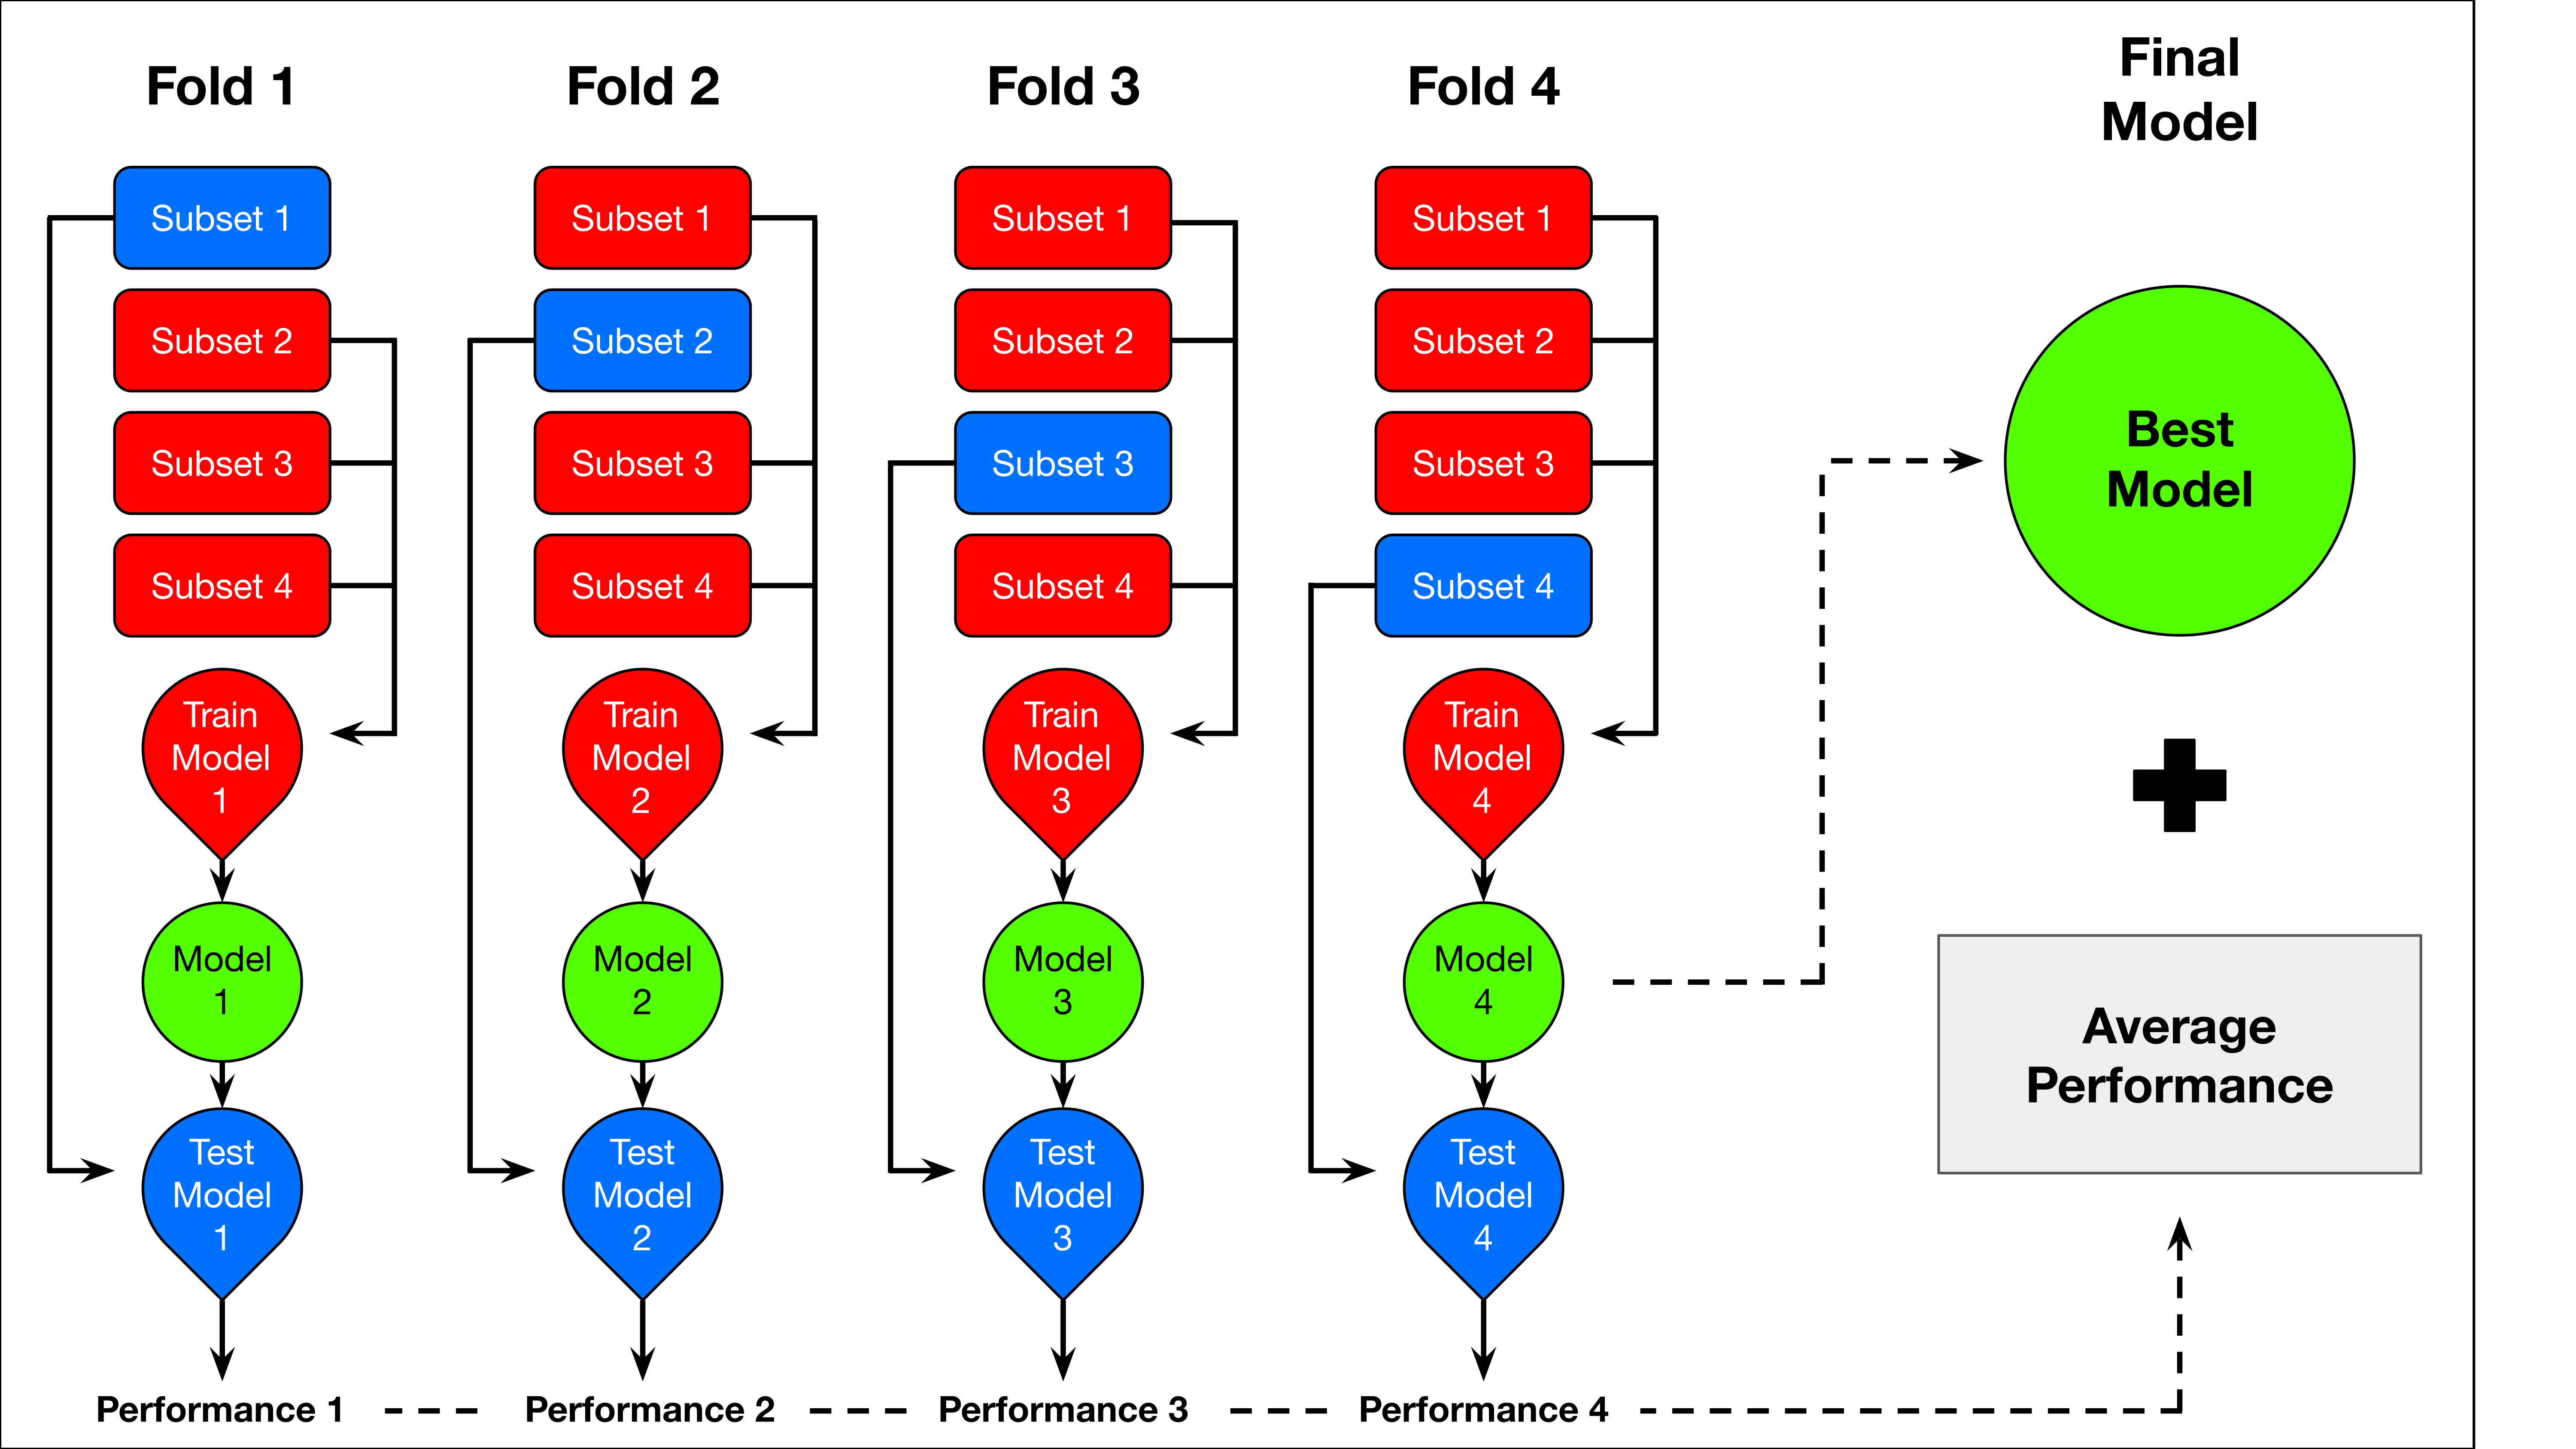
\includegraphics[width=62.5in,height=\textheight]{images/k-fold_fig.png}

}

\caption{\label{fig-k-fold}Schematic of \(k\)-fold cross validation. The
dataset is randomly divided into \(k\) stratified folds. Each fold
serves as the validation set once, while the remaining folds are
combined to create a training set for model development. Performance
metrics for the test set are calculated and recorded, and this process
is repeated for all \(k\) folds.}

\end{figure}%

\subsubsection{Feature Selection}\label{feature-selection}

Machine learning models are prone to overfitting, especially when
provided with a large set of predictive features (Ying, 2019).
Overfitting can degrade model performance on unseen data and increase
the demand for computational resources and memory storage (Li et al.,
2017). Dimensionality reduction offers a robust solution to these
challenges and generally falls into two broad categories: feature
extraction and feature selection.

Feature extraction involves transforming the original dataset into a
lower-dimensional feature space. However, this process generates new
features that often lack the physical interpretability of the original
variables. In contrast, feature selection identifies a subset of the
original features, preserving their physical meaning while improving
model readability and interpretability (Li et al., 2017). In this study,
supervised feature selection was employed to reduce the number of
predictors, which enhanced learning performance, reduced computational
costs, and mitigated overfitting.

To begin, an initial model was trained using the full feature set of 45
predictors (Table~\ref{tbl-predictors}). A feature selection method
based on feature importance was then applied to identify and remove less
relevant and noisy features. Feature importance scores quantify the
contribution of individual features---either positively or
negatively---to the model's predictions (Murdoch et al., 2019). In this
analysis, SHAP (SHapley Additive exPlanations) values were used to
compute feature importance scores (Lundberg \& Lee, 2017).

SHAP values is a method to explain the prediction of an individual
instance by calculating the contribution of each feature to that
prediction. The method is based on coalition game theory and is
discussed further in Lundberg \& Lee (2017). Here, SHAP values are used
for global interpretation of feature importance and feature effects on
the model. Global feature importance is produced by the absolute Shapley
values of each feature across the dataset, providing a list of features
in order of most to least important. Feature effects provide an
indication of the relationship between the value of a predicting feature
and its impact on the prediction.

The ten most important features Figure~\ref{fig-shap_values} were
selected based on their SHAP values and used to train a subsequent model
Table~\ref{tbl-predictors}. This refined model demonstrated improved
performance and reduced computational time compared to the initial
model. The final model, trained on this optimized feature subset, was
ultimately used for the analysis presented here.

\subsection{Statistical Analyses}\label{statistical-analyses}

Statistical analyses were conducted on annual BFI and base-flow values
from instrumented streamgages to identify temporal trends using the
Mann-Kendall nonparametric trend test (Kendall, 1970; Mann, 1945). This
test detects monotonic trends in datasets that are non-parametric and
assumes the absence of autocorrelation among observations. This test is
widely used in studies of this nature (Ayers et al., 2019; Ficklin et
al., 2016; Woodhouse et al., 2022).

To check for autocorrelation, we applied the Durbin-Watson test, which
revealed significant autocorrelation at four streamgages on an annual
basis. Of these, only one streamgage (09486500 - Santa Cruz River at
Cortaro, AZ) showed a significant trend in BFI. This streamgage was
excluded from the trend analysis, as autocorrelation could inflate the
variance of the Mann-Kendall statistic, potentially leading to biased
trend estimates (Hamed \& Rao, 1998). Trends with a \(\rho \le 0.05\)
are considered significant.

\section{Results}\label{results}

\subsection{BFI of Ungauged
Catchments}\label{bfi-of-ungauged-catchments}

\subsubsection{Model Validation}\label{model-validation}

Predicted values of BFI are plotted against observed values for the
entire period of record of the instrumented dataset in
Figure~\ref{fig-actual_predicted} . The agreement between ``out-of-bag''
predictions (blind cross-validation, treating each site as ungauged) and
observed values is acceptable (R\textsuperscript{2} = 0.764) indicating
that the model performs well across the full dataset. The overall RMSE
is 0.129 and the overall percent bias (pbias) is -5.6\%. Model
performance metrics across various classifications are summarized in
Table~\ref{tbl-performance}. These performance metrics demonstrate that
the regional model performs consistently well across different spatial
and climatic classifications. However, the negative pbias values across
all classifications, along with the overall pbias, indicate a systematic
underprediction of BFI by the model. Categories with relatively lower
R\textsuperscript{2} and Nash-Sutcliffe Efficiency (NSE) values also
exhibit higher biases, reflecting weaker model performance in those
specific contexts.

\begin{figure}

\centering{

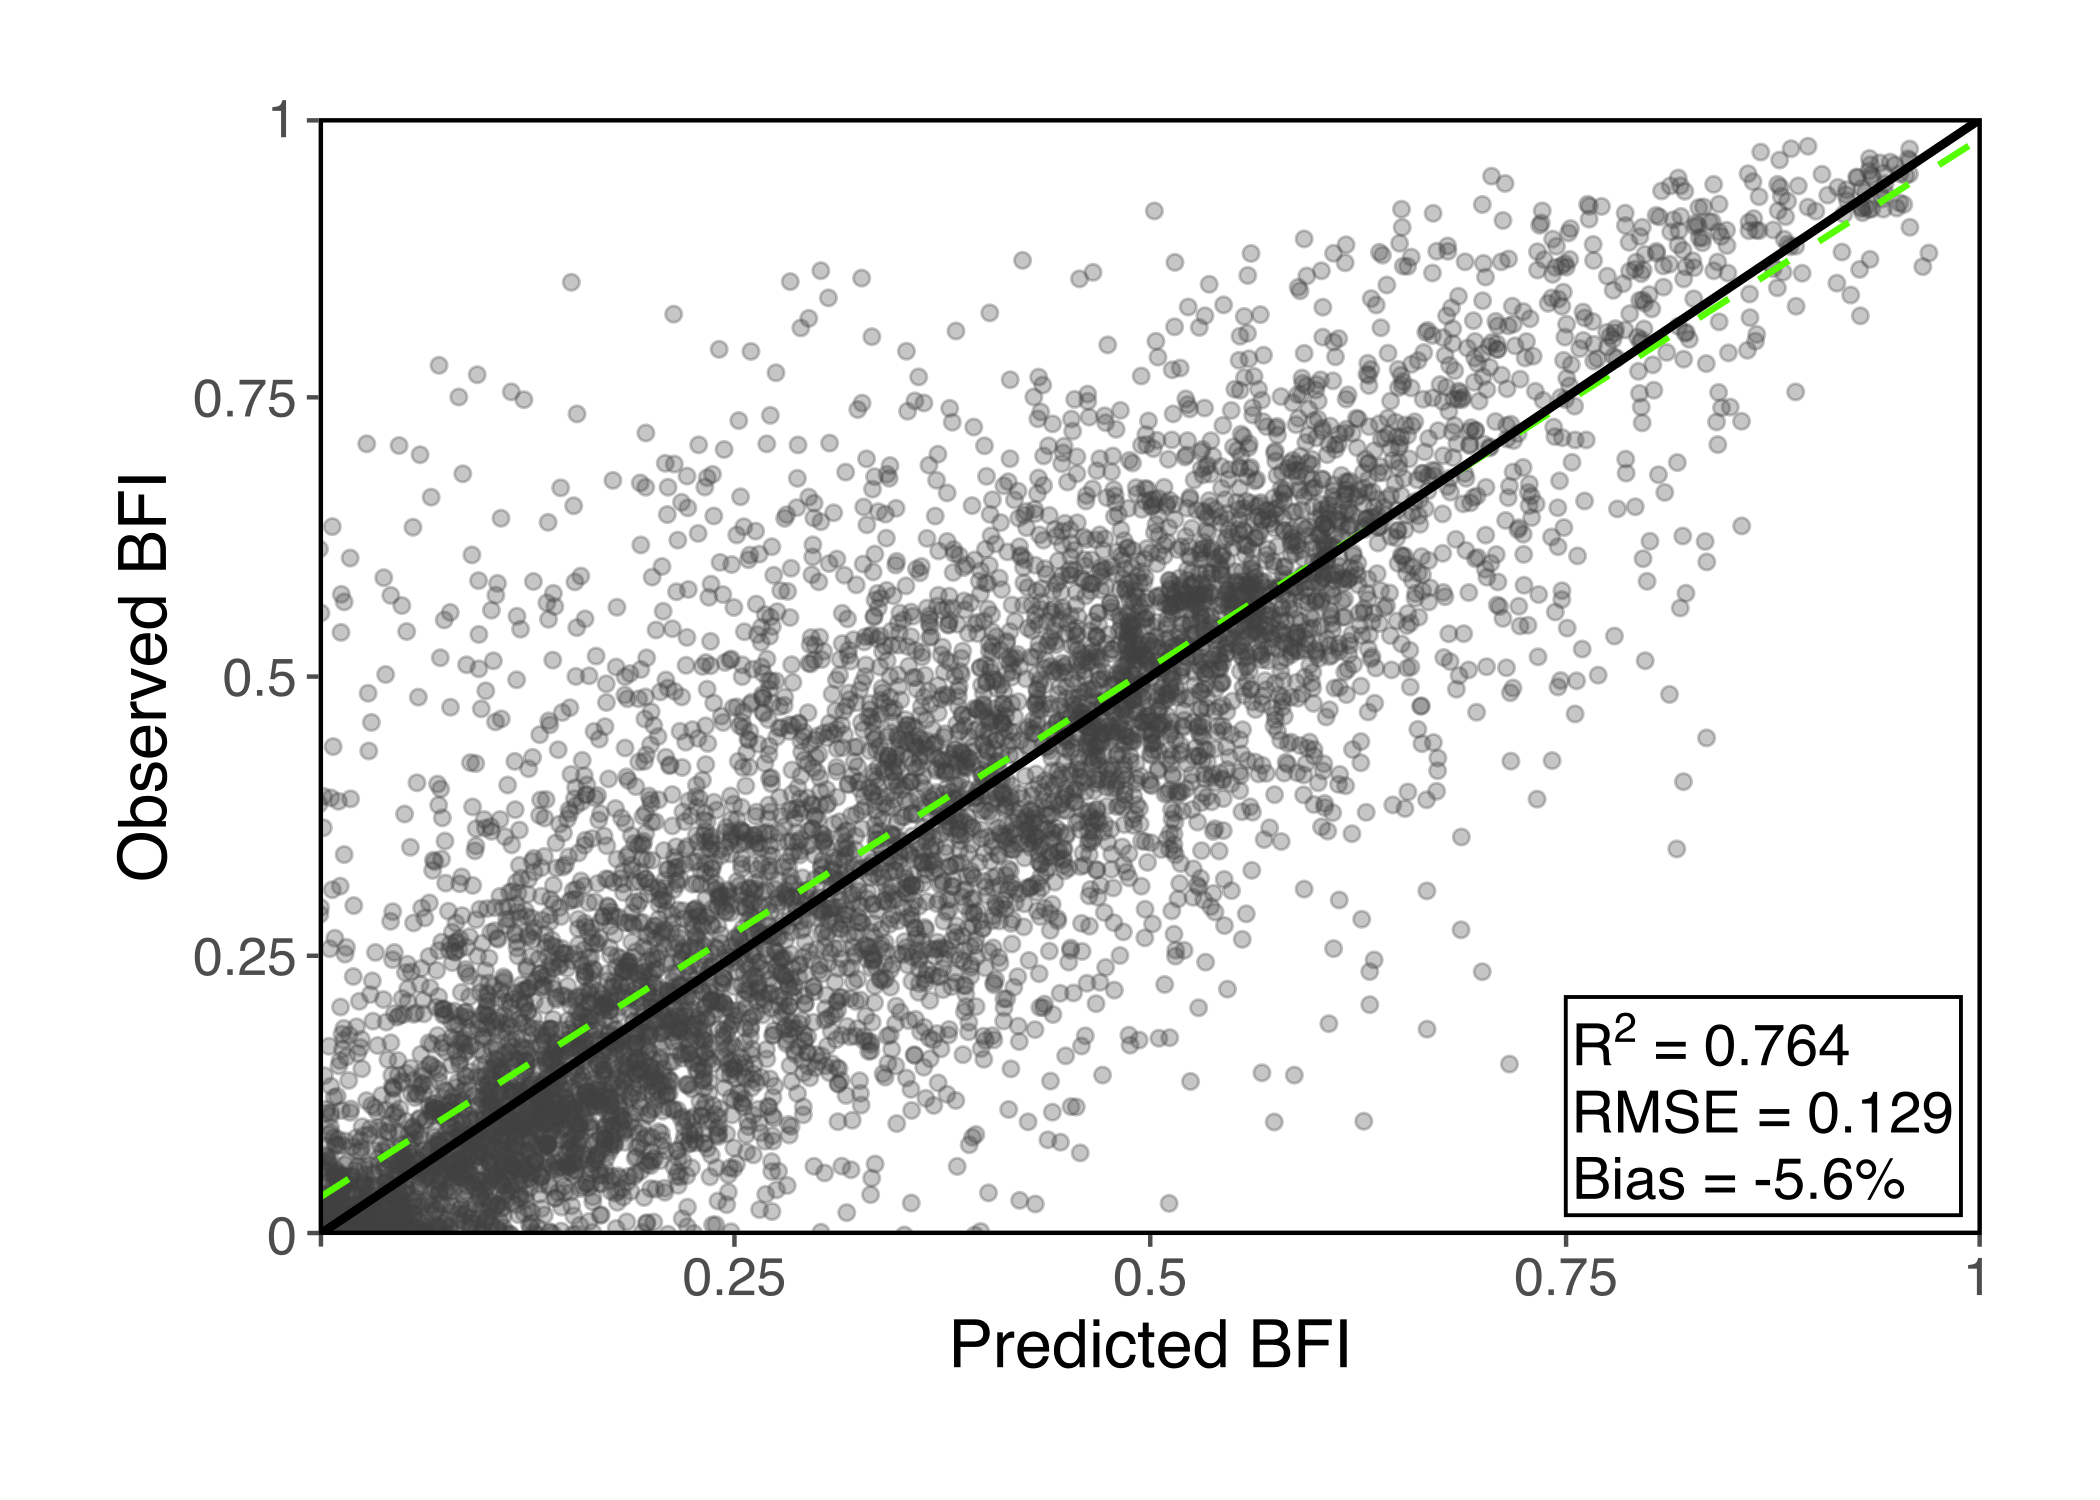
\includegraphics{images/actual-predicted.png}

}

\caption{\label{fig-actual_predicted}Linear relationship between
observed BFI and predicted BFI. The solid line is the 1:1 line, the
dashed line is regressed to the data.}

\end{figure}%

\begin{longtable}[]{@{}
  >{\raggedright\arraybackslash}p{(\columnwidth - 14\tabcolsep) * \real{0.1250}}
  >{\raggedright\arraybackslash}p{(\columnwidth - 14\tabcolsep) * \real{0.1250}}
  >{\raggedright\arraybackslash}p{(\columnwidth - 14\tabcolsep) * \real{0.1250}}
  >{\raggedright\arraybackslash}p{(\columnwidth - 14\tabcolsep) * \real{0.1250}}
  >{\raggedright\arraybackslash}p{(\columnwidth - 14\tabcolsep) * \real{0.1250}}
  >{\raggedright\arraybackslash}p{(\columnwidth - 14\tabcolsep) * \real{0.1250}}
  >{\raggedright\arraybackslash}p{(\columnwidth - 14\tabcolsep) * \real{0.1250}}
  >{\raggedright\arraybackslash}p{(\columnwidth - 14\tabcolsep) * \real{0.1250}}@{}}
\caption{Performance of model predictions for BFI for all sites split by
various classifications. n is number of observatios,
R\textsuperscript{2} is the coefficient of determination of a linear
regression, MSE is mean-squared-error, RMSE is root-mean-squared-error,
MAE is mean-absolute-error, NSE is Nash-Sucliffe efficiency, and pbias
is percent bias.}\label{tbl-performance}\tabularnewline
\toprule\noalign{}
\begin{minipage}[b]{\linewidth}\raggedright
\textbf{Classification Group}
\end{minipage} & \begin{minipage}[b]{\linewidth}\raggedright
\textbf{n}
\end{minipage} & \begin{minipage}[b]{\linewidth}\raggedright
\textbf{R2}
\end{minipage} & \begin{minipage}[b]{\linewidth}\raggedright
\textbf{MSE}
\end{minipage} & \begin{minipage}[b]{\linewidth}\raggedright
\textbf{RMSE}
\end{minipage} & \begin{minipage}[b]{\linewidth}\raggedright
\textbf{MAE}
\end{minipage} & \begin{minipage}[b]{\linewidth}\raggedright
\textbf{NSE}
\end{minipage} & \begin{minipage}[b]{\linewidth}\raggedright
\textbf{pbias}
\end{minipage} \\
\midrule\noalign{}
\endfirsthead
\toprule\noalign{}
\begin{minipage}[b]{\linewidth}\raggedright
\textbf{Classification Group}
\end{minipage} & \begin{minipage}[b]{\linewidth}\raggedright
\textbf{n}
\end{minipage} & \begin{minipage}[b]{\linewidth}\raggedright
\textbf{R2}
\end{minipage} & \begin{minipage}[b]{\linewidth}\raggedright
\textbf{MSE}
\end{minipage} & \begin{minipage}[b]{\linewidth}\raggedright
\textbf{RMSE}
\end{minipage} & \begin{minipage}[b]{\linewidth}\raggedright
\textbf{MAE}
\end{minipage} & \begin{minipage}[b]{\linewidth}\raggedright
\textbf{NSE}
\end{minipage} & \begin{minipage}[b]{\linewidth}\raggedright
\textbf{pbias}
\end{minipage} \\
\midrule\noalign{}
\endhead
\bottomrule\noalign{}
\endlastfoot
Climate - Monsoon Dominated & 3039 & 0.633 & 0.016 & 0.126 & 0.074 &
0.619 & -13.7 \\
Climate - Snowmelt Dominated & 4685 & 0.733 & 0.015 & 0.121 & 0.087 &
0.725 & -3.5 \\
PhysRegion - Basin\&Range & 6147 & 0.733 & 0.016 & 0.127 & 0.084 & 0.724
& -6.3 \\
PhysRegion - CO Plateau & 1577 & 0.846 & 0.011 & 0.104 & 0.073 & 0.843 &
-3.8 \\
Climate - Warm-Wet & 1506 & 0.693 & 0.014 & 0.117 & 0.077 & 0.685 &
-8.2 \\
Climate - Warm-Dry & 2351 & 0.693 & 0.022 & 0.147 & 0.092 & 0.675 &
-11.9 \\
Climate - Cool-Wet & 2350 & 0.738 & 0.011 & 0.106 & 0.078 & 0.736 &
-1.7 \\
Climate - Cool-Dry & 1517 & 0.831 & 0.012 & 0.111 & 0.078 & 0.827 &
-4.3 \\
Slope - High & 3795 & 0.776 & 0.012 & 0.111 & 0.079 & 0.771 & -3.3 \\
Slope - Low & 3929 & 0.724 & 0.018 & 0.133 & 0.085 & 0.713 & -9.1 \\
\end{longtable}

\subsubsection{Predictor Importance}\label{sec-predictor-importance}

The predictors used to estimate BFI at ungauged sites were evaluated for
their importance in the final XGBoost model, as illustrated in
Figure~\ref{fig-shap_values}. The most influential feature for
predicting long-term BFI is basin elevation. While elevation itself does
not directly affect base-flow characteristics, it has consistently been
identified as a key predictor in previous BFI studies (Beck et al.,
2013; Singh et al., 2018). The importance of elevation aligns with
findings from Beck et al. (2013), highlighting its role as a proxy for
climate variables such as temperature, precipitation, and snowpack
duration. Seasonal snowpack duration, in particular, has been shown to
strongly correlate with springflow and groundwater recharge in this
region (Donovan et al., 2022). This relationship is further supported by
hydroclimate features where higher temperatures tend to negatively
influence BFI, while precipitation exhibits a mixed influence. In some
cases, higher precipitation values correlate with lower BFI, likely due
to a larger proportion of precipitation contributing to runoff rather
than infiltration and groundwater recharge.

\begin{figure}

\centering{

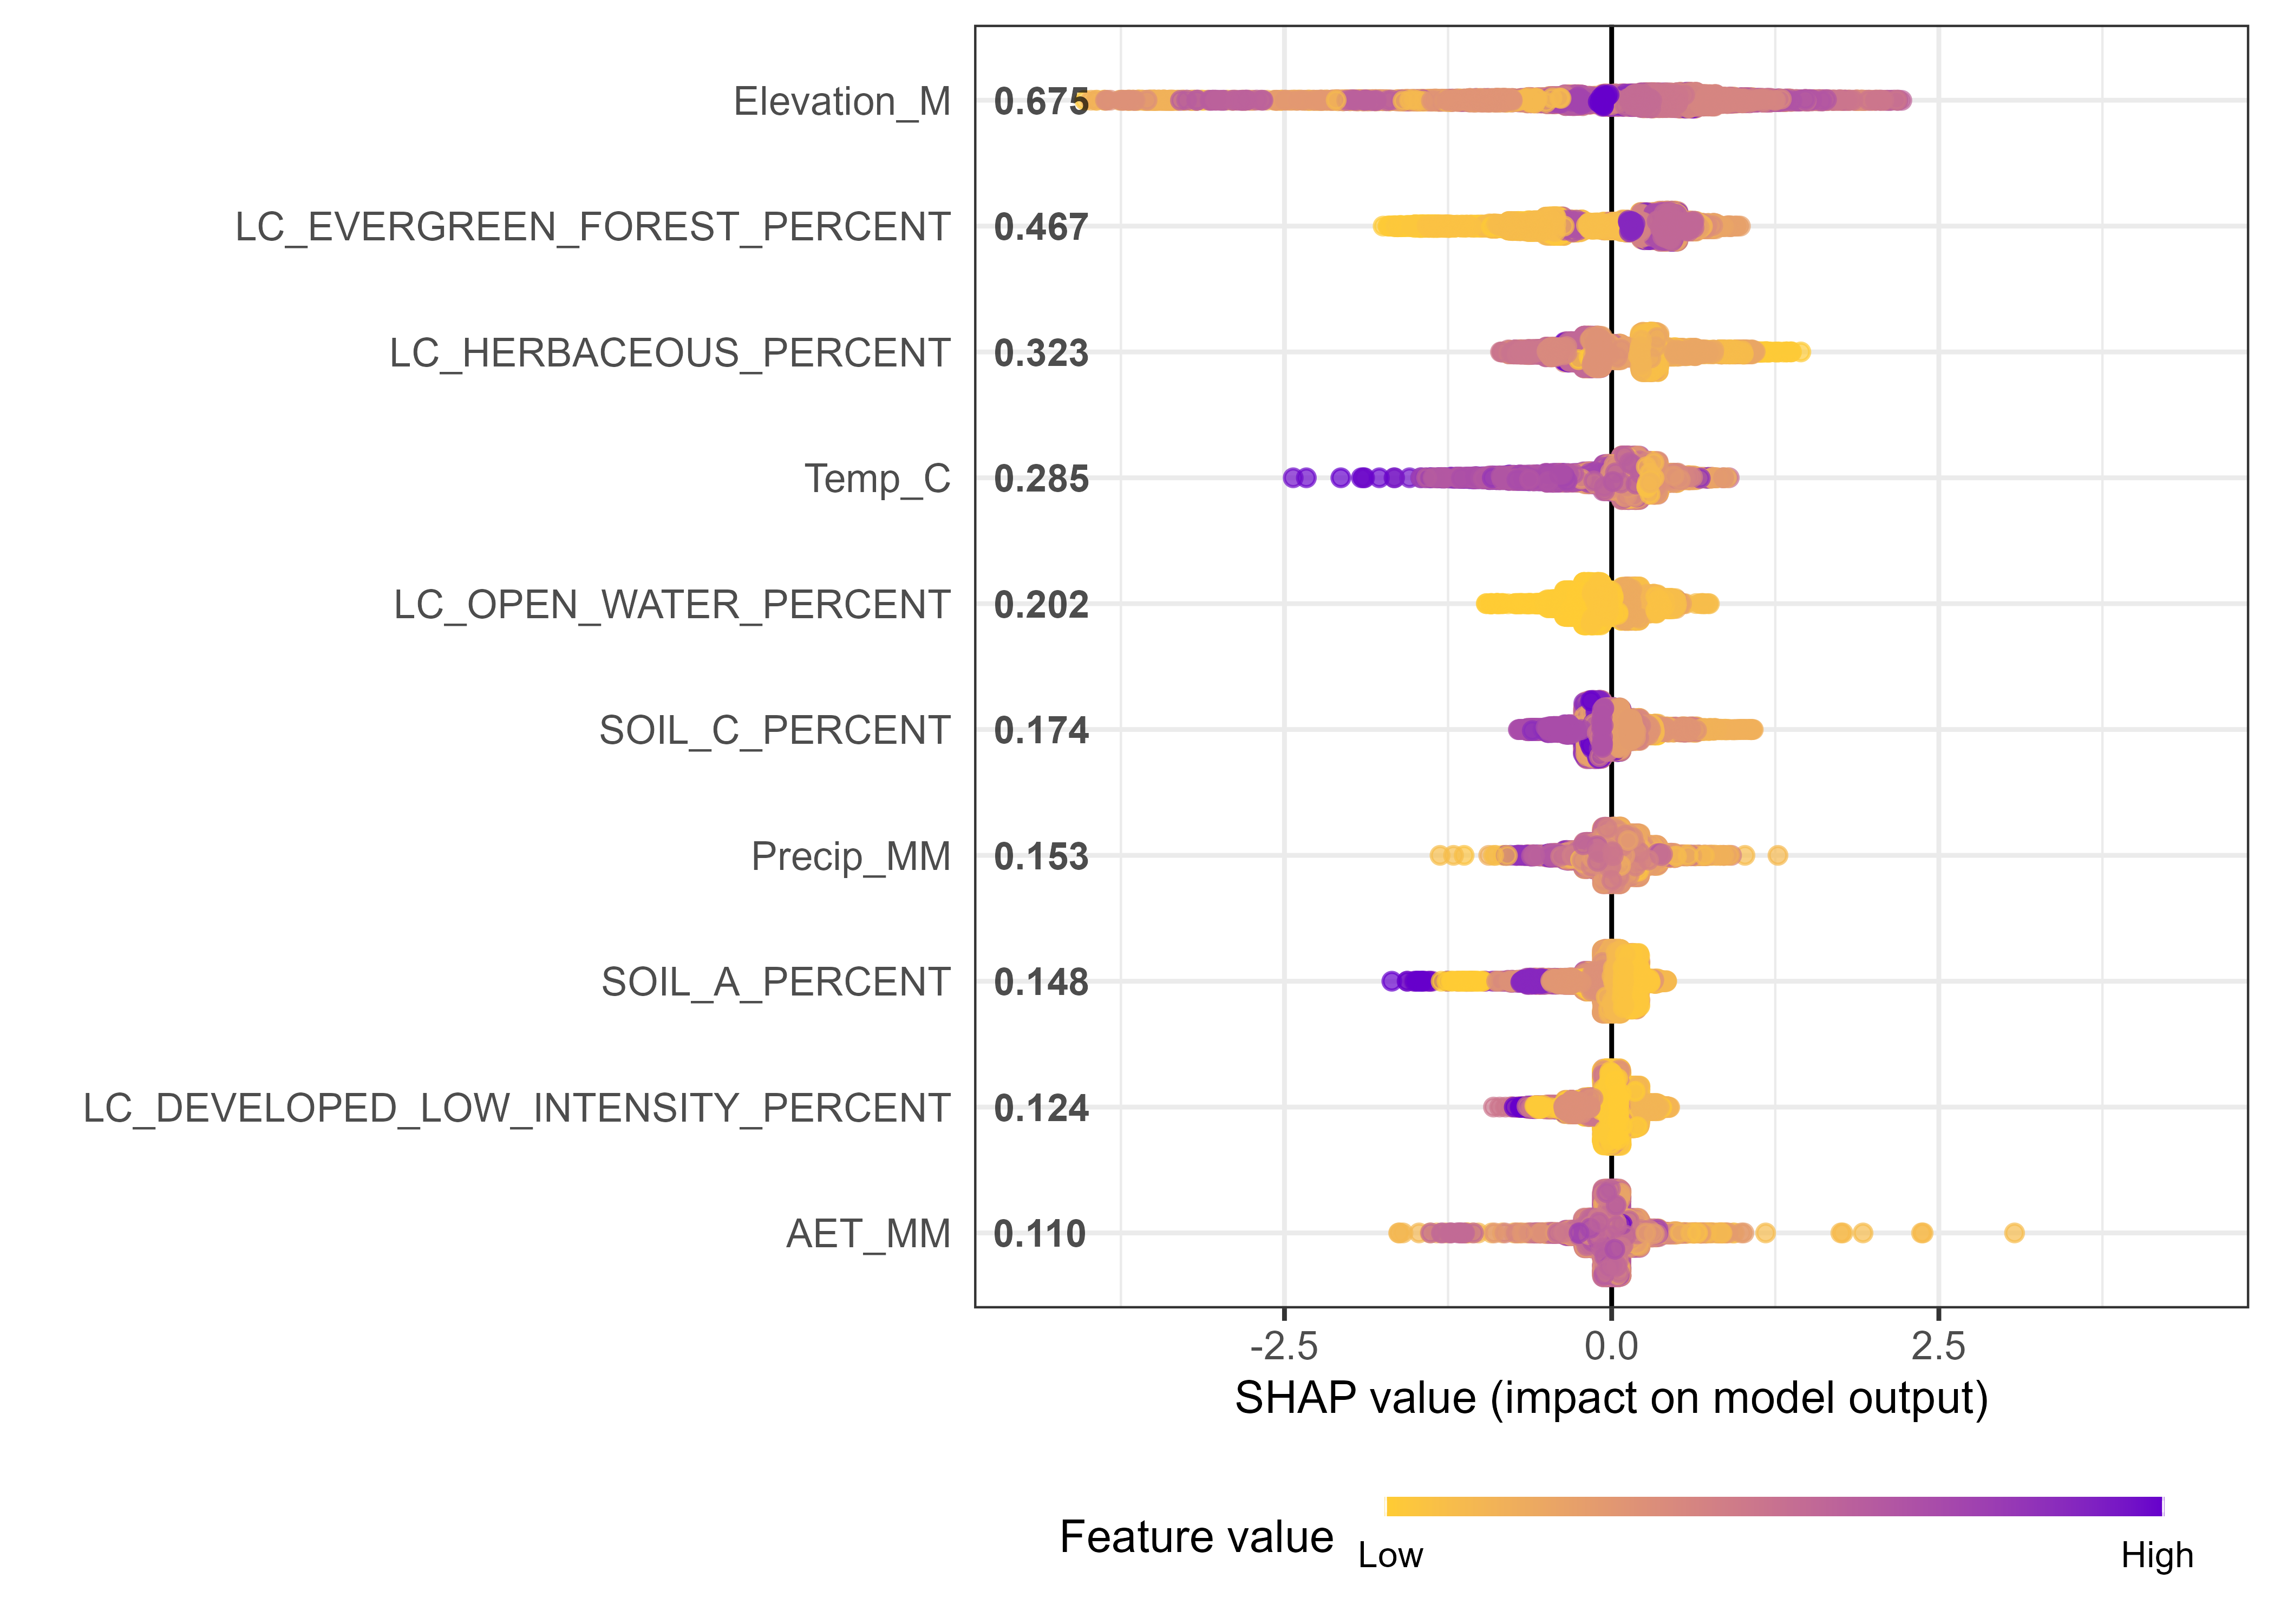
\includegraphics{images/shap_summary.png}

}

\caption{\label{fig-shap_values}SHAP value plot of features used in
final model. Land cover features are indicated by the percentage of
cover by each land cover type and soil types are defined by hydrologic
soil group.}

\end{figure}%

Land cover and land use predictors also play a significant role in BFI
estimation. Analysis of SHAP values indicates that a higher percentage
of evergreen forest positively influences BFI predictions, while higher
proportions of shrubland and developed land exert a negative influence.
Similarly, hydrologic soil types show distinct trends in their impact on
BFI. Soil Type C, characterized by moderately high runoff potential
(20-40\% clay), tends to negatively influence BFI. In contrast, Soil
Type A, which has low runoff potential and facilitates rapid water
infiltration, exhibits a mixed influence (USDA, 2009). The mixed effects
of Soil Type A are likely due to SHAP values capturing interactions
between features rather than direct relationships. For example, regions
dominated by Soil Type A may also have steep slopes or sparse
vegetation. Additionally, the relationship between Soil Type A and BFI
is likely non-linear and influenced by the complex dynamics of regional
base-flow processes.

\subsubsection{Predicted Long-term BFI}\label{predicted-long-term-bfi}

The regionalized (HUC-8) long-term BFI (1991--2020) is shown in
Figure~\ref{fig-bfi-huc}, while the long-term BFI for stream reaches
with a Strahler stream order of 3 or greater is presented in
Figure~\ref{fig-bfi-streams}. Basins with high BFIs, such as those along
the Grand Canyon in the northwestern part of the study area, indicate
greater surface water and groundwater interaction. Elevated BFI values
are also observed along portions of the Mogollon Rim, a heavily forested
region with high precipitation that marks the transition between
physiographic regions. Additionally, headwater regions of perennial
rivers tend to exhibit higher BFI values. In contrast, low BFI values
are found in areas like the Defiance Uplift in northeastern Arizona and
the arid southern regions of the state.

\begin{figure}

\centering{

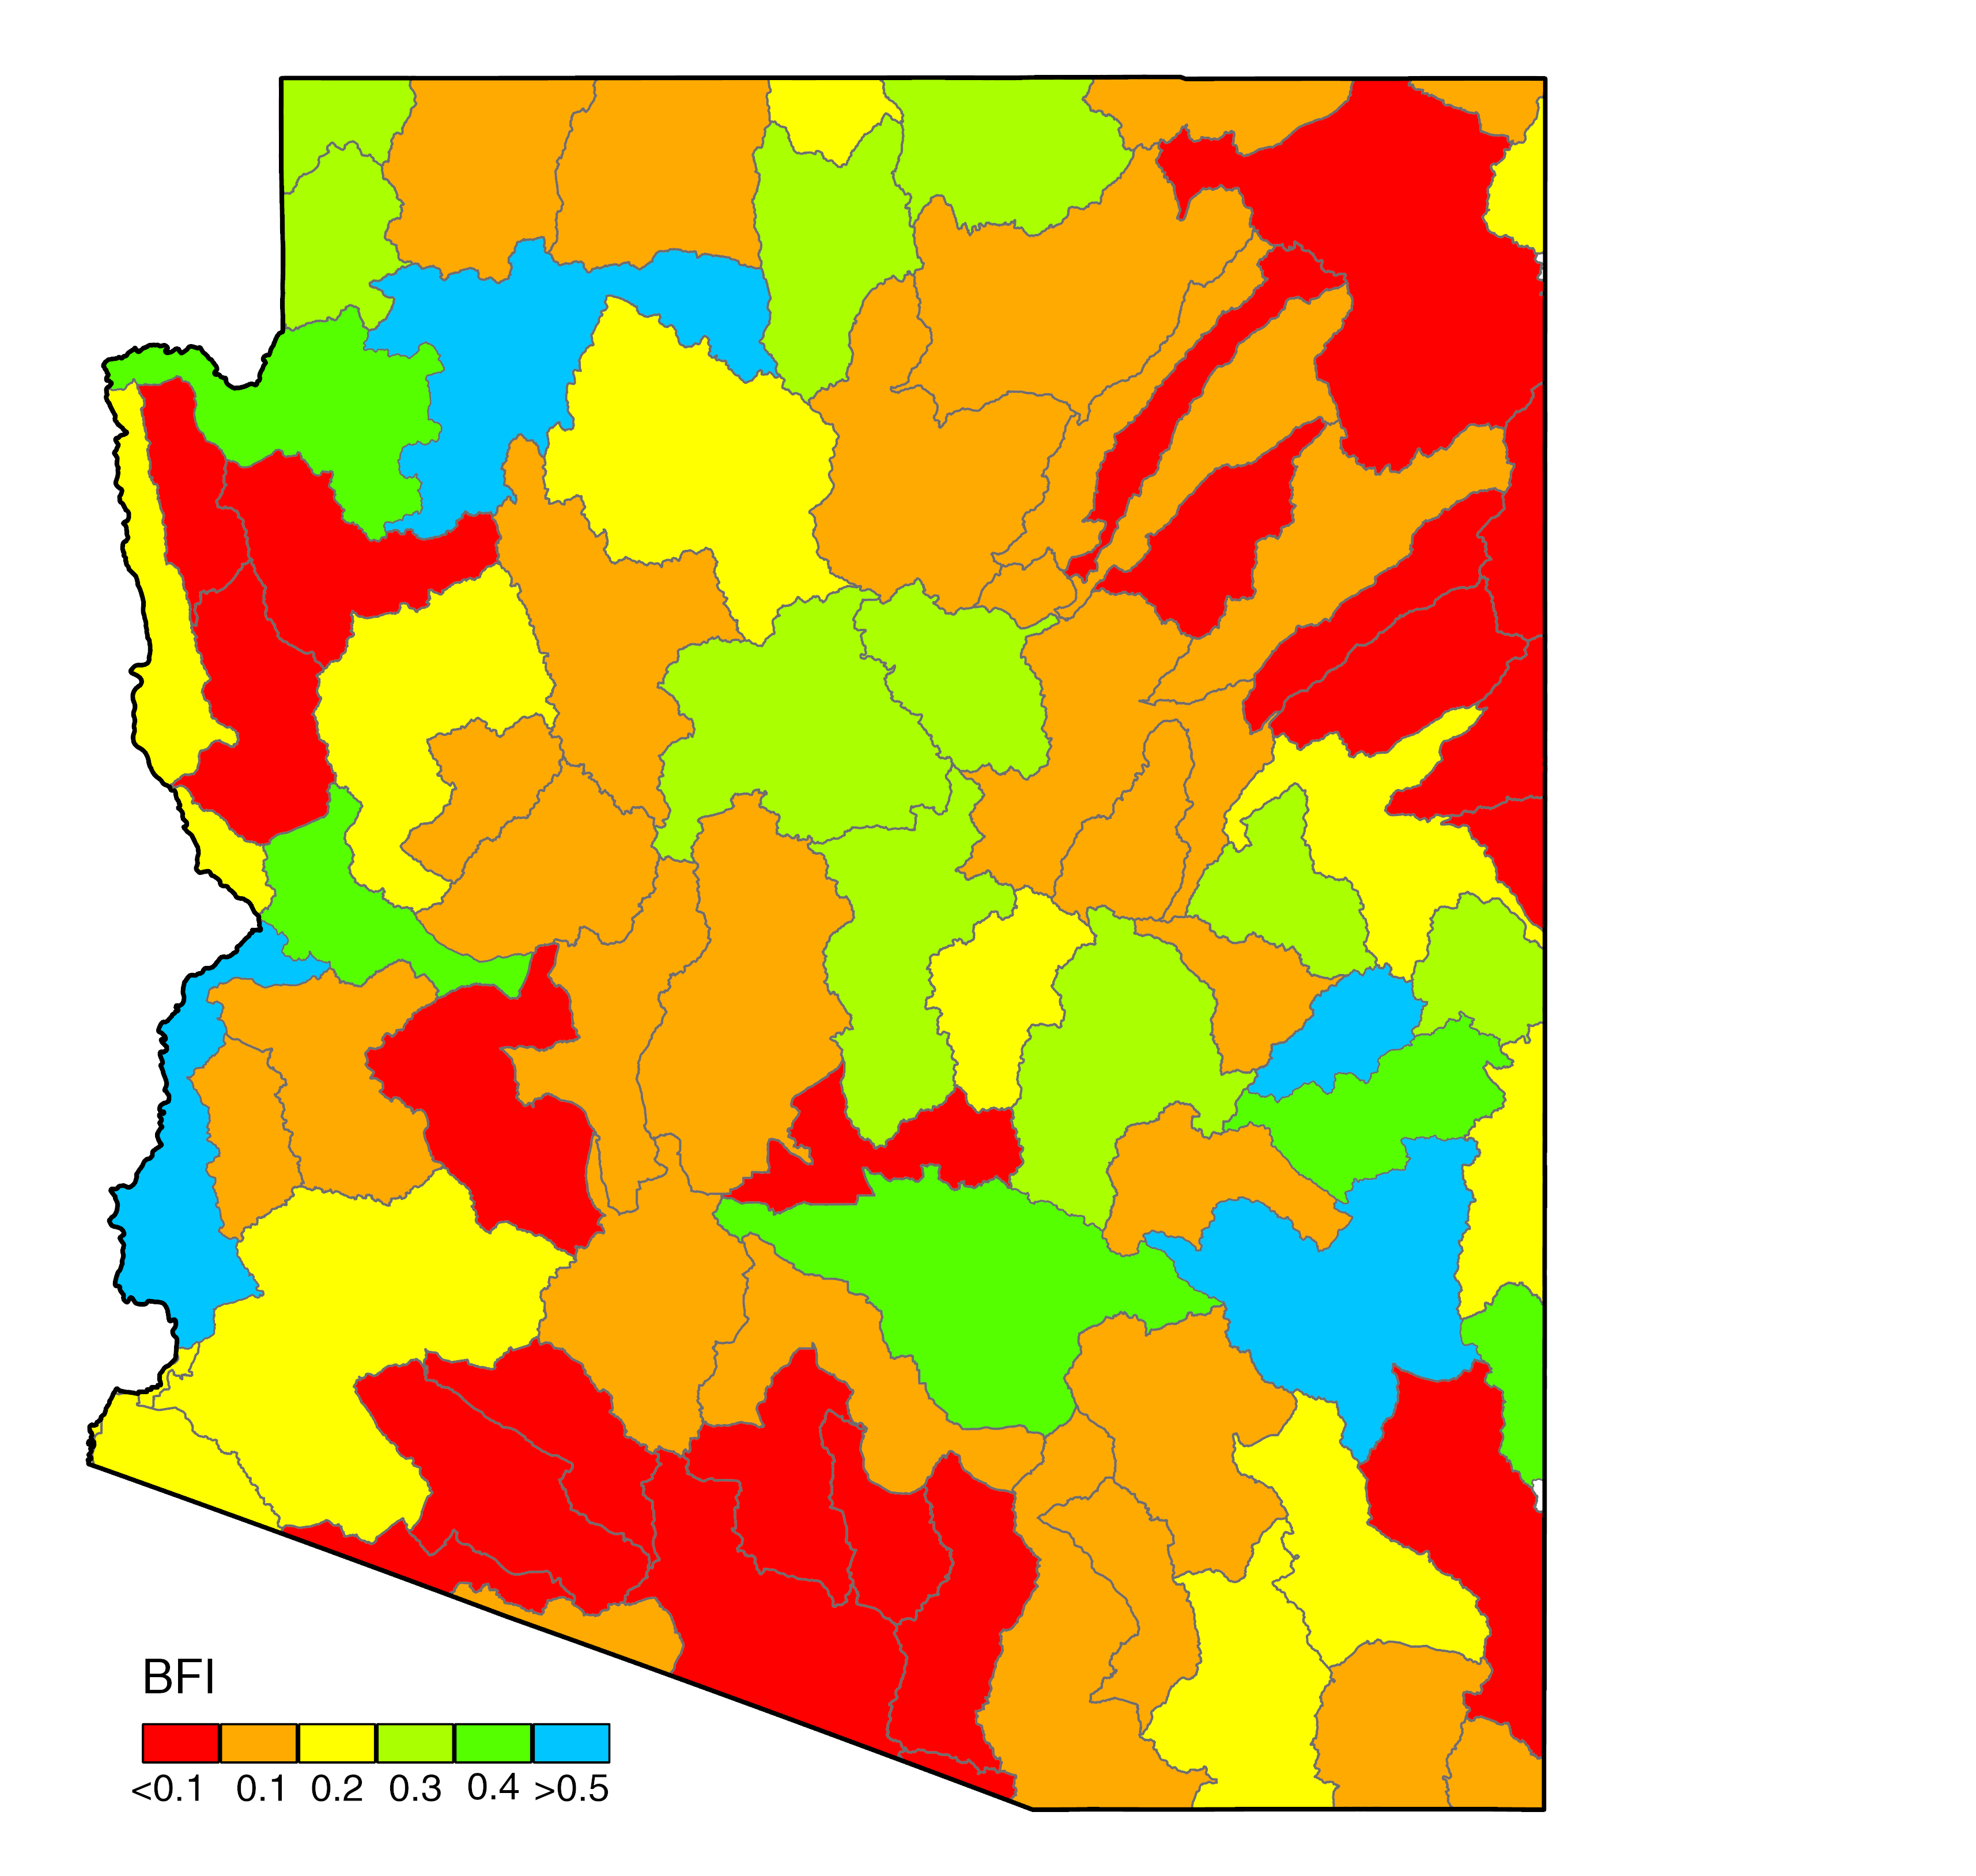
\includegraphics{images/BFI_HUC8_20241203.png}

}

\caption{\label{fig-bfi-huc}Predicted long-term BFI values for 8-digit
HUC (1991-2020)}

\end{figure}%

\begin{figure}

\centering{

\includegraphics{images/BFI_AllStream.png}

}

\caption{\label{fig-bfi-streams}Predicted long-term BFI values for all
stream reaches of Strahler stream order 3 and greater (1991-2020)}

\end{figure}%

Figure~\ref{fig-bfi-streams} indicates the predicted long-term BFI for
stream reaches in Arizona of a Strahler stream order of 3 or greater.
Stream-level BFI values often correspond to the long-term BFI observed
in HUC-8 basins, as geospatial predictor data were aggregated at the
basin level. Figure~\ref{fig-bfi-streams} highlights stream density
across the region, revealing areas with higher concentrations of
perennial streams, particularly in regions with favorable hydrogeologic
conditions, such as spring-fed systems in the Verde River and the Salt
River headwaters. Conversely, lower BFI values are observed in arid
regions and those with lower stream densities such as parts of the
Little Colorado River Basin, where groundwater recharge is limited
(Flint \& Flint, 2007). While BFI values and their spatial patterns may
align with certain terrain features or climatic patterns, it is
important to recognize that BFI is driven by complex interactions among
multiple factors Figure~\ref{fig-shap_values}.

\subsection{BFI of Gauged Catchments}\label{bfi-of-gauged-catchments}

\begin{figure}

\centering{

\includegraphics{images/BFI_Instrumented_20241203.png}

}

\caption{\label{fig-instrumented-bfi}Long-term BFI for the period of
record from instrumented stream flow data.}

\end{figure}%

The long-term BFI for the 205 gauged reaches across Arizona is
illustrated in Figure~\ref{fig-instrumented-bfi} . The long-term mean
BFI is 0.32, indicating that \textasciitilde32\% of long-term streamflow
in Arizona likely originates from groundwater discharge and other
delayed sources. The highest BFI values (\textgreater0.9) are found
along the Grand Canyon in northwestern Arizona. The highly karstic
geology of this region facilitates the rapid movement of subsurface flow
to surface water and spring outlets (Chambless et al., 2023). Relatively
high BFI values (\textgreater0.8) are found at the spring-fed headwaters
of the Verde River (Del Rio Spring) and the spring-fed headwaters of
Fossil Creek. These results are consistent with interpolated BFI values
reported by Wolock (2003).

The stream reaches of the Little Colorado River Basin (northeastern
Arizona) indicate consistently low BFI values (\textless{} 0.2). This is
likely due to low-yielding perched aquifers underlying the Defiance
Uplift in northeastern Arizona, which are hydrologically connected to
surface streams, while the high-yield, confined regional aquifer is much
deeper (Blanchard, 2002). A notable tendency emerges along most major
rivers in the study area: upstream reaches tend to exhibit higher BFI
values, while downstream reaches display lower values. This pattern is
presumed to result from greater groundwater-surface water interactions
at stream headwaters, influenced by spring outlets, and the dilution of
base flow as water moves downstream. This trend is particularly evident
along the Gila River, Verde River, and Little Colorado River in Arizona.

\subsubsection{Trends in Base Flow \& BFI}\label{sec-bfi-trends}

Trends in BFI over the period of record for each streamgage in this
analysis are illustrated in Figure~\ref{fig-instrumented-trend} and
Table~\ref{tbl-trends}. Base flow and BFI trends were analyzed across
all instrumented sites over their respective periods of record using the
Mann--Kendall test. Statistically significant trends were observed in
both metrics, with a 72.20\% coincidence rate between significant base
flow and BFI trends, indicating a strong dependence of BFI on base-flow
dynamics.

Figure~\ref{fig-instrumented-trend} illustrates the spatial variation in
BFI trends across the study area. Statistically significant decreasing
trends are observed at 16.1\% of sites, while increasing trends are
found at 8.8\% of sites, with no clear regional patterns for either. In
the Basin and Range physiographic region, 9\% of sites show increasing
trends, while 16.7\% exhibit decreasing trends. In the Colorado Plateau
region, increasing trends occur at 6.1\% of sites, and decreasing trends
are observed at 14.3\% of sites.

\begin{figure}

\centering{

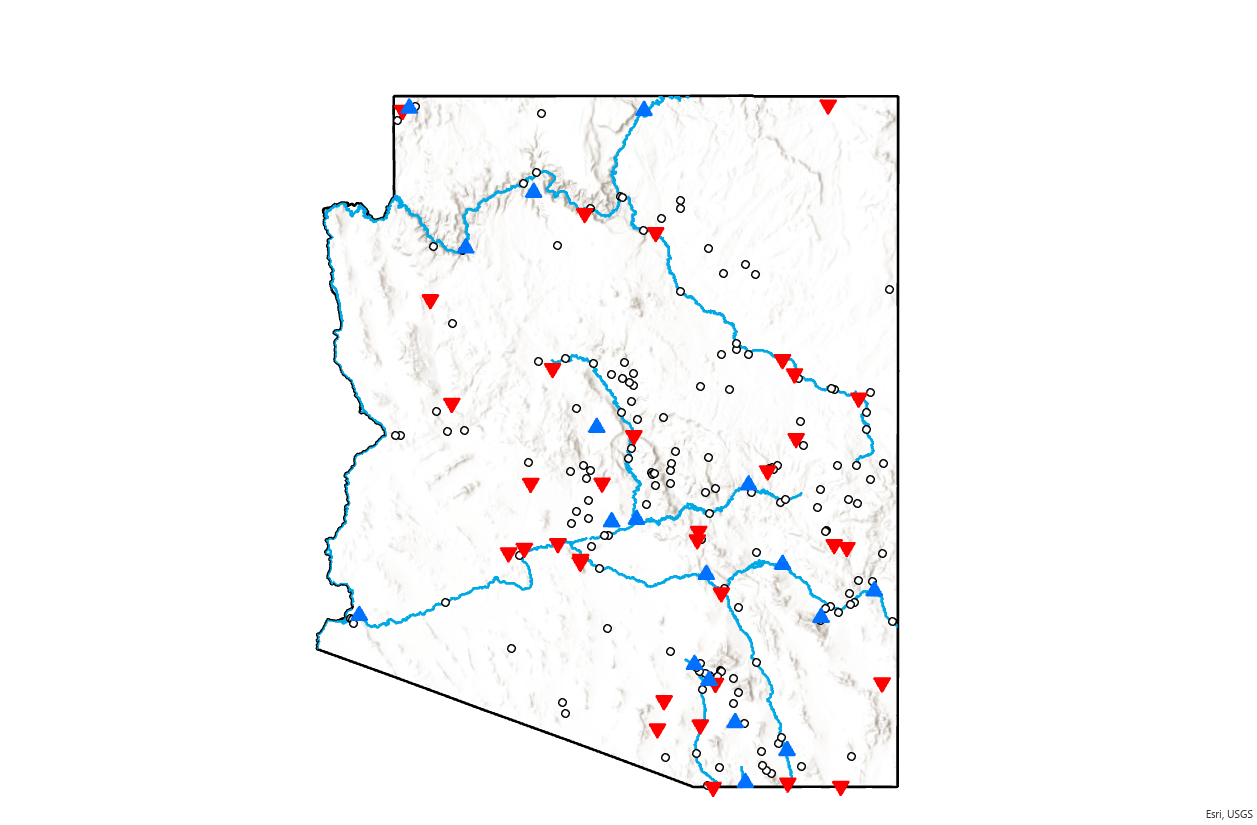
\includegraphics{images/BFITrends_20241203.png}

}

\caption{\label{fig-instrumented-trend}Trends in BFI over full period of
record for instrumented sites used in this study. Red upward (blue
downward) arrows indicate an increasing (decreasing) trend at a
significance level of 5\%. White circles represent sites with no
statistically significant trends.}

\end{figure}%

\subsubsection{Classification Trends}\label{classification-trends}

Classifications presented in Table~\ref{tbl-trends} were determined
based on precipitation regime, physiographic region, climate, and slope.
The dominant precipitation regime (monsoon vs.~snowmelt) was identified
by analyzing streamflow hydrographs for each station, focusing on peak
flow periods during the monsoon season (July--September) and the
snowmelt season (March--June). Physiographic region was assigned based
on which region the streamgage is located. Climate classifications were
defined as warm (above the long-term median temperature of Arizona),
cool (below the long-term median temperature), wet (above the long-term
median precipitation), and dry (below the long-term median
precipitation). Slope was categorized as high (above the median slope)
and low (below the median slope).

Statistically significant decreasing trends in BFI were more common than
increasing trends across all site classifications
(Table~\ref{tbl-trends}). While decreasing trends dominate, both
increasing and decreasing trends are observed within each
classification. Monsoon-dominated regions exhibit a higher proportion of
significant negative trends (24.1\%) compared to snowmelt-dominated
regions (10.2\%), suggesting that monsoon-dominated systems are more
consistently correlated with declining base flow. Among climate
classifications, warm-dry climates have the highest proportion of
negative trends (20.0\%), followed by warm-wet climates (19.4\%),
indicating that regions with higher temperatures are more prone to base
flow declines. Low-slope regions show a greater prevalence of negative
trends (20.4\%) compared to high-slope regions (11.8\%). This suggests
that flatter areas may be more susceptible to base-flow reductions,
potentially due to differences in hydrologic connectivity and recharge
dynamics.

\begin{longtable}[]{@{}
  >{\raggedright\arraybackslash}p{(\columnwidth - 10\tabcolsep) * \real{0.1667}}
  >{\raggedright\arraybackslash}p{(\columnwidth - 10\tabcolsep) * \real{0.1667}}
  >{\raggedright\arraybackslash}p{(\columnwidth - 10\tabcolsep) * \real{0.1667}}
  >{\raggedright\arraybackslash}p{(\columnwidth - 10\tabcolsep) * \real{0.1667}}
  >{\raggedright\arraybackslash}p{(\columnwidth - 10\tabcolsep) * \real{0.1667}}
  >{\raggedright\arraybackslash}p{(\columnwidth - 10\tabcolsep) * \real{0.1667}}@{}}
\caption{Comparison of trends for BFI for all sites split by various
classifications. Only sites with a significant (\(\rho \le 0.05\)) trend
are included here as established by a Mann-Kendall test for monotonic
trends across the full period of record. n is the number of sites,
n\_pos (n\_neg) is the number of sites with positive (negative) trends,
perc\_pos (perc\_neg) is the percentage of n with a positive (negative)
trend.}\label{tbl-trends}\tabularnewline
\toprule\noalign{}
\begin{minipage}[b]{\linewidth}\raggedright
\textbf{Classification Group}
\end{minipage} & \begin{minipage}[b]{\linewidth}\raggedright
\textbf{n}
\end{minipage} & \begin{minipage}[b]{\linewidth}\raggedright
\textbf{n\_pos}
\end{minipage} & \begin{minipage}[b]{\linewidth}\raggedright
\textbf{n\_neg}
\end{minipage} & \begin{minipage}[b]{\linewidth}\raggedright
\textbf{perc\_pos}
\end{minipage} & \begin{minipage}[b]{\linewidth}\raggedright
\textbf{perc\_neg}
\end{minipage} \\
\midrule\noalign{}
\endfirsthead
\toprule\noalign{}
\begin{minipage}[b]{\linewidth}\raggedright
\textbf{Classification Group}
\end{minipage} & \begin{minipage}[b]{\linewidth}\raggedright
\textbf{n}
\end{minipage} & \begin{minipage}[b]{\linewidth}\raggedright
\textbf{n\_pos}
\end{minipage} & \begin{minipage}[b]{\linewidth}\raggedright
\textbf{n\_neg}
\end{minipage} & \begin{minipage}[b]{\linewidth}\raggedright
\textbf{perc\_pos}
\end{minipage} & \begin{minipage}[b]{\linewidth}\raggedright
\textbf{perc\_neg}
\end{minipage} \\
\midrule\noalign{}
\endhead
\bottomrule\noalign{}
\endlastfoot
Precipitation - Monsoon Dominated & 87 & 8 & 21 & 0.092 & 0.241 \\
Precipitation - Snowmelt Dominated & 118 & 9 & 12 & 0.076 & 0.102 \\
Physiographic Region - Basin and Range & 156 & 14 & 26 & 0.090 &
0.167 \\
Physiographic Region - Colorado Plateau & 49 & 3 & 7 & 0.061 & 0.143 \\
Climate - Warm-Wet & 31 & 2 & 6 & 0.065 & 0.194 \\
Climate - Warm-Dry & 55 & 6 & 11 & 0.109 & 0.200 \\
Climate - Cool-Wet & 74 & 4 & 9 & 0.054 & 0.122 \\
Climate - Cool-Dry & 45 & 5 & 7 & 0.111 & 0.156 \\
Slope - High & 102 & 10 & 12 & 0.098 & 0.118 \\
Slope - Low & 103 & 7 & 21 & 0.068 & 0.204 \\
\end{longtable}

\subsubsection{Coincident Climate
Trends}\label{coincident-climate-trends}

Given the variations in the period of record across the instrumented
network (see SUPPLEMENTAL - Period of Record figure), we analyzed trends
in base flow and BFI in relation to coincident trends in climate
variables. Trends are classified as coincident when the direction of the
climate variable trend (positive or negative) aligns with the trend
observed in base flow or BFI (Table~\ref{tbl-coincident-trends}). This
analysis includes both significant and non-significant trends, which is
appropriate where the influence of complex, interconnected processes may
not always manifest as statistically significant patterns over limited
observational periods (Ficklin et al., 2016).

\begin{longtable}[]{@{}lcc@{}}
\caption{Coincident trends of climate variables (ET\textsubscript{O},
precipitation, temperature) with base flow and BFI
trends.}\label{tbl-coincident-trends}\tabularnewline
\toprule\noalign{}
& \textbf{Climate Variable} & \textbf{Coincidence Percentage (\%)} \\
\midrule\noalign{}
\endfirsthead
\toprule\noalign{}
& \textbf{Climate Variable} & \textbf{Coincidence Percentage (\%)} \\
\midrule\noalign{}
\endhead
\bottomrule\noalign{}
\endlastfoot
BFI & ET\textsubscript{O} & 44.88 \\
& Precipitation & 53.17 \\
& Temperature & 47.32 \\
Base Flow & ET\textsubscript{O} & 55.12 \\
& Precipitation & 64.88 \\
& Temperature & 39.02 \\
\end{longtable}

The analysis shows that base flow and BFI trends most frequently align
with precipitation trends (64.88\% and 53.17\%, respectively),
emphasizing precipitation as the primary driver of local groundwater
recharge and discharge. Coincidence with ET\textsubscript{O} (reference
evapotranspiration) trends (55.12\% for base flow and 44.88\% for BFI)
suggests that evapotranspiration also plays a significant role,
particularly in arid regions where it can reduce recharge or base flow
during dry periods. In contrast, temperature trends show lower
percentages of coincidence, often opposing base flow and BFI trends.
Specifically, positive (negative) temperature trends are frequently
associated with negative (positive) base-flow trends (60.98\%) and BFI
trends (52.68\%). These results highlight the complex interplay between
climatic variables and hydrological processes. While precipitation
exerts the strongest influence on base flow and BFI, evapotranspiration
and temperature add further variability in specific environmental
contexts.

\section{Summary \& Conclusions}\label{sec-conclusion}

This study provides new insights into base-flow dynamics and groundwater
contributions in Arizona's dryland rivers by combining an analysis of
instrumented streamflow records with machine learning predictions for
ungauged basins. The results highlight significant spatial variability
in BFI, with approximately 32\% of Arizona's long-term streamflow
originating from groundwater discharge. Regions such as the Grand Canyon
and Mogollon Rim demonstrate high BFI values due to strong
groundwater-surface water interactions, while areas like the Little
Colorado River Basin exhibit low BFI values, reflecting limited
groundwater recharge.

Using an XGBoost machine learning algorithm, we successfully predicted
long-term BFI in ungauged basins, achieving strong model performance (R²
= 0.764, RMSE = 0.129). The model performed well across all
classifications, demonstrating its robustness in capturing base-flow
dynamics across a region with substantial variability in climate,
elevation, and physiographic characteristics. Key predictors included
elevation, land cover, and soil type, highlighting the importance of
integrating hydroclimate and physiographic characteristics into regional
hydrological models. These predictions address the limitations posed by
Arizona's sparse streamgage network, offering a scalable approach to
estimate BFI in data-limited regions.

Our analysis of BFI trends in gauged catchments revealed that
precipitation is the primary driver of base-flow variability, with
evapotranspiration and temperature contributing additional complexity.
These findings emphasize the critical role of climate-hydrology
interactions in shaping groundwater contributions to streamflow. Inverse
trends between temperature and BFI suggest that further warming could
reduce groundwater contributions to streamflow. Coincident trends in
precipitation and BFI further underscore the importance of understanding
recharge processes, especially in arid and semi-arid landscapes, where
precipitation events play key roles in replenishing groundwater.

However, the utility of the streamgage networks for base-flow analyses
in Arizona is limited by their design and focus. There has been an
increase in the number of streamgages in the region to meet regulatory
imperatives, such as the Clean Water Act. Even so, many of these gages
are not suited for base-flow studies because they emphasize peak flow
monitoring and lack the ability to accurately measure low-flow dynamics
(Maricopa County, 2020). New, non-USGS streamgages are typically
installed by flood control districts (e.g.~the ALERT system) and are
designed for tracking flood flows rather than base flow. New USGS
streamgages have been added over the past decade to address instream
flow rights and to improve the density of monitoring in the future.

This study demonstrates the benefits of combining observational records
with machine learning to improve our understanding of streamflow
processes in drylands. Future work should explore the projected effects
of climate change on base-flow processes and developing models for other
data-poor regions. The framework presented here has broad applicability
to other arid and semi-arid regions worldwide and can inform water
resource management strategies aimed at addressing water scarcity and
adapting to climate variability.

\section*{References}\label{references}
\addcontentsline{toc}{section}{References}

\phantomsection\label{refs}
\begin{CSLReferences}{1}{0}
\bibitem[\citeproctext]{ref-abatzoglou2018}
Abatzoglou, J. T. et al. (2018). TerraClimate, a high-resolution global
dataset of monthly climate and climatic water balance from
1958{\textendash}2015. \emph{Scientific Data}, \emph{5}(1), 170191.
\url{https://doi.org/10.1038/sdata.2017.191}

\bibitem[\citeproctext]{ref-ahiablame2013}
Ahiablame, L. et al. (2013). Estimation of annual baseflow at ungauged
sites in Indiana USA. \emph{Journal of Hydrology}, \emph{476}, 13--27.
\url{https://doi.org/10.1016/j.jhydrol.2012.10.002}

\bibitem[\citeproctext]{ref-az_climate2024}
Arizona State Climate Office. (2024). {Climate of Arizona}. Retrieved
from \url{https://globalfutures.asu.edu/azclimate/climate/}

\bibitem[\citeproctext]{ref-arnold1995}
Arnold, J. G. et al. (1995). Automated Base Flow Separation and
Recession Analysis Techniques. \emph{Ground Water}, \emph{33}(6),
1010--1018. \url{https://doi.org/10.1111/j.1745-6584.1995.tb00046.x}

\bibitem[\citeproctext]{ref-ARNOLD200021}
Arnold, J. G. et al. (2000). Regional estimation of base flow and
groundwater recharge in the upper mississippi river basin. \emph{Journal
of Hydrology}, \emph{227}(1), 21--40.
https://doi.org/\url{https://doi.org/10.1016/S0022-1694(99)00139-0}

\bibitem[\citeproctext]{ref-ayers2019}
Ayers, J. R., Villarini, G., Jones, C., \& Schilling, K. (2019). Changes
in monthly baseflow across the U.S. Midwest. \emph{Hydrological
Processes}, \emph{33}(5), 748--758.
\url{https://doi.org/10.1002/hyp.13359}

\bibitem[\citeproctext]{ref-beck2013}
Beck, H. E. et al. (2013). Global patterns in base flow index and
recession based on streamflow observations from 3394 catchments: Global
Patterns in Base Flow Characteristics. \emph{Water Resources Research},
\emph{49}(12), 7843--7863. \url{https://doi.org/10.1002/2013WR013918}

\bibitem[\citeproctext]{ref-blanchard02}
Blanchard, P. J. (2002). \emph{Assessments of aquifer sensitivity on
{Navajo Nation} and adjacent lands and ground-water vulnerability to
pesticide contamination on the {Navajo Indian Irrigation Project},
{Arizona}, {New Mexico}, and {Utah}} (No. Water-Resources Investigations
Report 02-4051). {USGS}. \url{https://doi.org/10.3133/wri024051}

\bibitem[\citeproctext]{ref-bloomfield2009}
Bloomfield, J. P. et al. (2009). Examining geological controls on
baseflow index (BFI) using regression analysis: An illustration from the
Thames Basin, UK. \emph{Journal of Hydrology}, \emph{373}(1-2),
164--176. \url{https://doi.org/10.1016/j.jhydrol.2009.04.025}

\bibitem[\citeproctext]{ref-bosch2017}
Bosch, D. D. et al. (2017). Temporal variations in baseflow for the
Little River experimental watershed in South Georgia, USA. \emph{Journal
of Hydrology: Regional Studies}, \emph{10}, 110--121.
\url{https://doi.org/10.1016/j.ejrh.2017.02.002}

\bibitem[\citeproctext]{ref-buban_PRISM}
Buban, M. S. et al. (2020). A comparison of the u.s. Climate reference
network precipitation data to the parameter-elevation regressions on
independent slopes model (PRISM). \emph{Journal of Hydrometeorology},
\emph{21}(10), 2391--2400. \url{https://doi.org/10.1175/JHM-D-19-0232.1}

\bibitem[\citeproctext]{ref-chambless_deep-karst_2023}
Chambless, H. E. et al. (2023). Deep-karst aquifer spring-flow trends in
a water-limited system, grand canyon national park, {USA}.
\emph{Hydrogeology Journal}, \emph{31}(7), 1755--1771.
\url{https://doi.org/10.1007/s10040-023-02702-w}

\bibitem[\citeproctext]{ref-chen2016xgboost}
Chen, T. et al. (2016). Xgboost: A scalable tree boosting system. In
\emph{Proceedings of the 22nd acm sigkdd international conference on
knowledge discovery and data mining} (pp. 785--794).

\bibitem[\citeproctext]{ref-daly2008}
Daly, C. et al. (2008). Physiographically sensitive mapping of
climatological temperature and precipitation across the conterminous
United States. \emph{International Journal of Climatology},
\emph{28}(15), 2031--2064. \url{https://doi.org/10.1002/joc.1688}

\bibitem[\citeproctext]{ref-donovan_karst_2022}
Donovan, K. M. et al. (2022). Karst spring processes and storage
implications in high elevation, semiarid southwestern united states. In
M. J. Currell \& B. G. Katz (Eds.), \emph{Geophysical monograph series}
(1st ed., pp. 35--50). Wiley.
\url{https://doi.org/10.1002/9781119818625.ch4}

\bibitem[\citeproctext]{ref-eastoe2019mtnblock}
Eastoe, C. J. et al. (2019). Hydrology of mountain blocks in arizona and
new mexico as revealed by isotopes in groundwater and precipitation.
\emph{Geosciences}, \emph{9}(11).
\url{https://doi.org/10.3390/geosciences9110461}

\bibitem[\citeproctext]{ref-eckhardt2005}
Eckhardt, K. (2005). How to construct recursive digital filters for
baseflow separation. \emph{Hydrological Processes}, \emph{19}(2),
507--515. \url{https://doi.org/10.1002/hyp.5675}

\bibitem[\citeproctext]{ref-eckhardt2008}
Eckhardt, K. (2008). A comparison of baseflow indices, which were
calculated with seven different baseflow separation methods.
\emph{Journal of Hydrology}, \emph{352}(1-2), 168--173.
\url{https://doi.org/10.1016/j.jhydrol.2008.01.005}

\bibitem[\citeproctext]{ref-eckhardt2023}
Eckhardt, K. (2023). Technical note: How physically based is hydrograph
separation by recursive digital filtering? \emph{Hydrology and Earth
System Sciences}, \emph{27}(2), 495--499.
\url{https://doi.org/10.5194/hess-27-495-2023}

\bibitem[\citeproctext]{ref-fekete2007}
Fekete, B. M. et al. (2007). The current status of global river
discharge monitoring and potential new technologies complementing
traditional discharge measurements.

\bibitem[\citeproctext]{ref-ficklin2016}
Ficklin, D. L. et al. (2016). Impacts of recent climate change on trends
in baseflow and stormflow in United States watersheds. \emph{Geophysical
Research Letters}, \emph{43}(10), 5079--5088.
\url{https://doi.org/10.1002/2016GL069121}

\bibitem[\citeproctext]{ref-flint_flint07}
Flint, L. E., \& Flint, A. L. (2007). \emph{Regional Analysis of
Ground-Water Recharge}.

\bibitem[\citeproctext]{ref-fuka2014ecohydrology}
Fuka, D. et al. (2014). EcoHydRology: A community modeling foundation
for eco-hydrology. \emph{R Package Version 0.4}, \emph{12}.

\bibitem[\citeproctext]{ref-Georganos2018Very}
Georganos, S. et al. (2018). Very high resolution object-based land
use--land cover urban classification using extreme gradient boosting.
\emph{IEEE Geoscience and Remote Sensing Letters}, \emph{15}, 607--611.
\url{https://doi.org/10.1109/LGRS.2018.2803259}

\bibitem[\citeproctext]{ref-gonzales2009}
Gonzales, A. L. et al. (2009). Comparison of different base flow
separation methods in a lowland catchment. \emph{Hydrology and Earth
System Sciences}, \emph{13}(11), 2055--2068.
\url{https://doi.org/10.5194/hess-13-2055-2009}

\bibitem[\citeproctext]{ref-MK_Hamed1998}
Hamed, K. H., \& Rao, A. (1998). A modified mann-kendall trend test for
autocorrelated data. \emph{Journal of Hydrology}, \emph{204}(1),
182--196.
https://doi.org/\url{https://doi.org/10.1016/S0022-1694(97)00125-X}

\bibitem[\citeproctext]{ref-instituteofhydrology1980}
Institute of Hydrology. (1980). \emph{Low flow studies report 3
catchment characteristic estimation manual}.

\bibitem[\citeproctext]{ref-iucn-drylands-2019}
IUCN. (2019, September). Drylands and climate change. Retrieved from
\url{https://www.iucn.org/resources/issues-brief/drylands-and-climate-change}

\bibitem[\citeproctext]{ref-kendall1970}
Kendall, M. G. (1970). \emph{Rank correlation methods} (4th ed). London:
Griffin.

\bibitem[\citeproctext]{ref-epa_AZephemeral}
Levick, L. R. et al. (2008). {The ecological and hydrological
significance of ephemeral and intermittent streams in the arid and
semi-arid American Southwest}. \emph{U.S. Environmental Protection
Agency and USDA/ARS Southwest Watershed Research Center},
(EPA/600/R-08/134).

\bibitem[\citeproctext]{ref-feat_selec2017}
Li, J., Cheng, K., Wang, S., Morstatter, F., Trevino, R. P., Tang, J.,
\& Liu, H. (2017). Feature selection: A data perspective. \emph{ACM
Comput. Surv.}, \emph{50}(6). \url{https://doi.org/10.1145/3136625}

\bibitem[\citeproctext]{ref-SHAP_values}
Lundberg, S. M., \& Lee, S.-I. (2017). A unified approach to
interpreting model predictions, \emph{30}. Retrieved from
\url{https://proceedings.neurips.cc/paper_files/paper/2017/file/8a20a8621978632d76c43dfd28b67767-Paper.pdf}

\bibitem[\citeproctext]{ref-lyne1979}
Lyne, V. et al. (1979). Institute of engineers australia national
conference. In (Vol. 79, pp. 89--93). Barton, Australia: Institute of
Engineers Australia.

\bibitem[\citeproctext]{ref-mann1945nonparametric}
Mann, H. B. (1945). Nonparametric tests against trend.
\emph{Econometrica: Journal of the Econometric Society}, 245--259.

\bibitem[\citeproctext]{ref-flood-control2020}
Maricopa County, F. C. D. of. (2020). \emph{{Flood Warning Program -
Program Review}}. Maricopa County Flood Control District. Retrieved from
\url{https://alert.fcd.maricopa.gov/alert/FWP_report_FINAL.pdf}

\bibitem[\citeproctext]{ref-ML_interpretability2019}
Murdoch, W. J., Singh, C., Kumbier, K., Abbasi-Asl, R., \& Yu, B.
(2019). Definitions, methods, and applications in interpretable machine
learning. \emph{Proceedings of the National Academy of Sciences},
\emph{116}(44), 22071--22080.
\url{https://doi.org/10.1073/pnas.1900654116}

\bibitem[\citeproctext]{ref-nathan1990}
Nathan, R. J. et al. (1990). Evaluation of automated techniques for base
flow and recession analyses. \emph{Water Resources Research},
\emph{26}(7), 1465--1473. \url{https://doi.org/10.1029/WR026i007p01465}

\bibitem[\citeproctext]{ref-neff2005}
Neff, B. P. et al. (2005). \emph{Base flow in the great lakes basin}
(Report No. 2005-5217). Reston, VA.
\url{https://doi.org/10.3133/sir20055217}

\bibitem[\citeproctext]{ref-ni2020streamflow}
Ni, L. et al. (2020). Streamflow forecasting using extreme gradient
boosting model coupled with gaussian mixture model. \emph{Journal of
Hydrology}, \emph{586}, 124901.

\bibitem[\citeproctext]{ref-odonnell2016}
O'Donnell, F. C. et al. (2016). 12th Biennial Conference of Research on
the Colorado Plateau. In.

\bibitem[\citeproctext]{ref-reitz2017}
Reitz, M. et al. (2017). Annual Estimates of Recharge, Quick{-}Flow
Runoff, and Evapotranspiration for the Contiguous US Using Empirical
Regression Equations. \emph{JAWRA Journal of the American Water
Resources Association}, \emph{53}(4), 961--983.
\url{https://doi.org/10.1111/1752-1688.12546}

\bibitem[\citeproctext]{ref-Rozos2021Machine}
Rozos, E. et al. (2021). Machine learning in assessing the performance
of hydrological models. \emph{Hydrology}.
\url{https://doi.org/10.3390/hydrology9010005}

\bibitem[\citeproctext]{ref-santhi2008}
Santhi, C. et al. (2008). Regional estimation of base flow for the
conterminous United States by hydrologic landscape regions.
\emph{Journal of Hydrology}, \emph{351}(1-2), 139--153.
\url{https://doi.org/10.1016/j.jhydrol.2007.12.018}

\bibitem[\citeproctext]{ref-scanlon2006}
Scanlon, B. R. et al. (2006). Global synthesis of groundwater recharge
in semiarid and arid regions. \emph{Hydrological Processes},
\emph{20}(15), 3335--3370. \url{https://doi.org/10.1002/hyp.6335}

\bibitem[\citeproctext]{ref-schmidt_ML_2020}
Schmidt, L. et al. (2020). Challenges in applying machine learning
models for hydrological inference: A case study for flooding events
across germany. \emph{Water Resources Research}, \emph{56}(5),
e2019WR025924.
https://doi.org/\url{https://doi.org/10.1029/2019WR025924}

\bibitem[\citeproctext]{ref-sheppard2002}
Sheppard, P. et al. (2002). The climate of the US Southwest.
\emph{Climate Research}, \emph{21}, 219--238.
\url{https://doi.org/10.3354/cr021219}

\bibitem[\citeproctext]{ref-singh2018}
Singh, S. K. et al. (2018). Towards baseflow index characterisation at
national scale in New Zealand. \emph{Journal of Hydrology}, \emph{568},
646--657. \url{https://doi.org/10.1016/j.jhydrol.2018.11.025}

\bibitem[\citeproctext]{ref-sloto1996}
Sloto, R. et al. (1996). \emph{HYSEP: A Computer Program for Streamflow
Hydrograph Separation and Analysis} (No. 96-4040). {USGS}.
\url{https://doi.org/10.3133/wri964040}

\bibitem[\citeproctext]{ref-szczepanek2022daily}
Szczepanek, R. (2022). Daily streamflow forecasting in mountainous
catchment using XGBoost, LightGBM and CatBoost. \emph{Hydrology},
\emph{9}(12), 226.

\bibitem[\citeproctext]{ref-tan2020}
Tan, X. et al. (2020). Global Changes in Baseflow Under the Impacts of
Changing Climate and Vegetation. \emph{Water Resources Research},
\emph{56}(9), e2020WR027349. \url{https://doi.org/10.1029/2020WR027349}

\bibitem[\citeproctext]{ref-taylor2013}
Taylor, R. G. et al. (2013). Ground water and climate change.
\emph{Nature Climate Change}, \emph{3}(4), 322--329.
\url{https://doi.org/10.1038/nclimate1744}

\bibitem[\citeproctext]{ref-nrcs2009}
USDA. (2009). \emph{Part 630 hydrology national engineering handbook,
chapter 7: Hydrologic soil groups}. USDA Natural Resources Conservation
Service.

\bibitem[\citeproctext]{ref-usgs2010}
USGS. (2010). Water resources data for the united states water year
2007. \url{http://wdr.water.usgs.gov/wy2007/search.jsp}.

\bibitem[\citeproctext]{ref-usgs-glossary-2018}
USGS. (2018). Water science glossary. Retrieved from
\url{https://www.usgs.gov/special-topics/water-science-school/science/water-science-glossary}

\bibitem[\citeproctext]{ref-wolock2003}
Wolock, D. M. (2003). Estimated mean annual natural ground-water
recharge in the conterminous united states.
\url{https://doi.org/10.5066/P9FSSVF3}.

\bibitem[\citeproctext]{ref-woodhouse_udall22}
Woodhouse, C. A. et al. (2022). Upper {Gila}, {Salt}, and {Verde
Rivers}: {Arid Land Rivers} in a {Changing Climate}. \emph{Earth
Interactions}, \emph{26}(1), 1--14.
\url{https://doi.org/10.1175/EI-D-21-0014.1}

\bibitem[\citeproctext]{ref-yao2018}
Yao, Y. et al. (2018). Role of Groundwater in the Dryland
Ecohydrological System: A Case Study of the Heihe River Basin.
\emph{Journal of Geophysical Research: Atmospheres}, \emph{123}(13),
6760--6776. \url{https://doi.org/10.1029/2018JD028432}

\bibitem[\citeproctext]{ref-Ying_2019}
Ying, X. (2019). An overview of overfitting and its solutions.
\emph{Journal of Physics: Conference Series}, \emph{1168}(2), 022022.
\url{https://doi.org/10.1088/1742-6596/1168/2/022022}

\bibitem[\citeproctext]{ref-zomer2022}
Zomer, R. J. et al. (2022). Version 3 of the Global Aridity Index and
Potential Evapotranspiration Database. \emph{Scientific Data},
\emph{9}(1), 409. \url{https://doi.org/10.1038/s41597-022-01493-1}

\end{CSLReferences}




\end{document}
